%----------------------------------------------------------------------------------------
%	PACKAGES AND DOCUMENT CONFIGURATIONS
%----------------------------------------------------------------------------------------

% !TeX spellcheck = it
\documentclass[11pt, a4paper, hidelinks]{report}

\usepackage{anyfontsize}
%\usepackage{siunitx} % Provides the \SI{}{} and \si{} command for typesetting SI units
\usepackage{graphicx} % Required for the inclusion of images
\usepackage{subcaption}
\usepackage[round]{natbib} % Required to change bibliography style to APA
\usepackage{amsmath} % Required for some math elements
\usepackage[export]{adjustbox}
\usepackage{eurosym} % euro simbol
\usepackage{hyperref} % hyperlink
\usepackage[utf8]{inputenc}
\usepackage{bookmark}
\usepackage{float} % to fix images in the document flow
\usepackage{epigraph}
\usepackage{quoting} % to create citations
\usepackage{newlfont}
\usepackage{color}
\usepackage[a4paper, total={6.2in, 8in}]{geometry}
\usepackage{algorithm2e} % pseudocode
\usepackage{algorithmic} % pseudocode
\usepackage{titletoc}
\usepackage{listings} % code
\usepackage{seqsplit} % split long lines

\bibliographystyle{plainnat}

\hypersetup{
  colorlinks=true,
  urlcolor=red,
  linkcolor=black,
  citecolor=blue
}

% Code style
\lstdefinestyle{mystyle}{
    basicstyle=\ttfamily\footnotesize,
    breakatwhitespace=false,
    breaklines=true,
    captionpos=b,
    keepspaces=true,
    % numbers=left,
    % numbersep=5pt,
	language=Python,
    showspaces=false,
    showstringspaces=false,
    showtabs=false,
    tabsize=2
}

\lstset{style=mystyle}

% To add numbers in algorithm lines
\LinesNumbered

\renewcommand{\labelenumi}{\alph{enumi}.} % Make numbering in the enumerate environment by letter rather than number (e.g. section 6)

% Remove Chapter N from the document preserving the numbering
\makeatletter
\def\@makechapterhead#1{%
  \vspace*{50\p@}%
  {\parindent \z@ \raggedright \normalfont
    \ifnum \c@secnumdepth >\m@ne
      %\if@mainmatter
        %\huge\bfseries \@chapapp\space \thechapter
        \Huge\bfseries \thechapter.\space%
        %\par\nobreak
        %\vskip 20\p@
      %\fi
    \fi
    \interlinepenalty\@M
    \Huge \bfseries #1\par\nobreak
    \vskip 40\p@
  }}
\makeatother


\begin{document}
\begin{titlepage}

\begin{center}
{{\Large{\textsc{Alma Mater Studiorum $\cdot$ University of Bologna}}}}
\rule[0.1cm]{15.8cm}{0.25mm}
\\\vspace{3mm}
%
%
{\Large{Dipartimento di Informatica - Scienza e Ingegneria\\
Artificial Intelligence}}


\end{center}

\vspace{20mm}

\begin{center}{
%
%
	{\LARGE{\textbf{Flatland Challenge}}}}
\end{center}

\vspace{15mm}

{\begin{center}
	 \large{Project Presentation}
\end{center}}

\vspace{32mm} \par \noindent

\begin{minipage}[t]{0.47\textwidth}
%
%
{\large{ Professor \vspace{2mm}\\{\textbf{Andrea Asperti}
}\\\\\\}}
\end{minipage}
%
\hfill
%
\begin{minipage}[t]{0.47\textwidth}\raggedleft{}{
{\large{ Students
\vspace{2mm}\\
\textbf{Alessandro Lombardi\\Fiorenzo Parascandolo}}}}
\end{minipage}

\vspace{31mm}

\begin{center}
Academic Year {2019-2020}
\end{center}

\end{titlepage}

{\tableofcontents}
\thispagestyle{empty}

\newpage
\setcounter{page}{1}

\chapter{Introduction}

The \href{https://www.aicrowd.com/challenges/neurips-2020-flatland-challenge/}{Flatland Challenge} aims to address the problem of train scheduling and rescheduling by providing a simple grid world environment and allowing for diverse experimental approaches.
The following work is related to the second edition of this challenge started in Summer 2020.
In the first edition, which took place in 2019, the majority of the participants delivered solutions from the operations research field, this edition tries to encourage participants to elaborate Reinforcement Learning solutions, indeed the challenge has been selected to be featured in the \href{https://neurips.cc/Conferences/2020/CompetitionTrack}{NeurIPS 2020 Accepted competitions}.
In this work we propose and describe the implementation of some Deep Reinforcement Learning solutions, leveraging the most recent outcomes in this vibrant and exciting field of study.

\chapter{Flatland environment}\label{ch:flatland-environment}

In order to conceive a solution for this challenge we need to fully understand the environment, how does it work and how do some subtle details influence behind the scenes what we can only perceive through observations and rewards.
The following results have been evaluated on the Python package \href{https://pypi.org/project/flatland-rl/}{flatland-rl version 2.1.10}.

\section{The classes RailAgentStatus and EnvAgent}\label{sec:the-classes-railagentstatus-and-envagent}

\textbf{RailAgentStatus} extends Python IntEnum and assumes the following values:
\begin{itemize}
	\item READY\_TO\_DEPART (0) the agent is not in the grid yet (position is None).
If a MOVE\_* action is performed during this state it becomes ACTIVE\@.
	\item ACTIVE (1) the agent is in the grid (position is not None) and hasn't reached the target yet.
	\item DONE (2) the agent is still in the grid (position is not None) but has already reached the target.
	\item DONE\_REMOVED (3) the agent has reached the target and has been removed from the grid.
\end{itemize}

\textbf{Grid4TransitionsEnum} extends Python standard IntEnum and assumes the following values: NORTH (0), EAST (1), SOUTH (2), WEST (3).
\textbf{Grid4TransitionsEnum} is used to indicate absolute directions (like a compass), related to the environment and not to the agents' orientations.
Possible usages are storing where an agent is facing or computing legal actions, for example including in the observations a one hot encoding representing the directions where an agent can move.
\\
\textbf{EnvAgent} class models the agent and encapsulates in its internal state the following attributes:
\begin{itemize}
	\item initial\_position: Tuple[int, int], initial coordinate.
	\item initial\_direction: Grid4TransitionsEnum, the initial agent facing direction.
	\item direction: Grid4TransitionsEnum, the current facing direction.
	\item target: Tuple[int, int], the final coordinate.
	\item moving: bool, True if the agent is in a moving state.
	\item speed\_data: dictionary, containing information about the agent's speed.
	\item malfunction\_data: dictionary, containing information about malfunctions.
	\item status: RailAgentStatus, the current agent status.
\end{itemize}

The speed of an agent contains the keys 'position\_fraction' used as a counter of the percentage of completion of an movement from a cell to another, 'speed' the value between 0 and 1 used to increment the 'position\_fraction' and 'transition\_action\_on\_cellexit' which contains the action to perform on the next cell, if it completes the one in the current step, otherwise in following steps may change multiple times.

The malfunction of an agent contains the keys 'malfunction' which contains how many steps are necessary to fix the agent, 'malfunction\_rate', the mean rate (average number of events in an interval) of the Poisson distribution, 'next\_malfunction' the number of steps the next malfunction will occur and 'nr\_malfunctions' the number of previous malfunctions.

\section{The class RailEnv}\label{sec:the-class-railenv}

From the documentation
\begin{quotation}
	RailEnv is an environment inspired by a (simplified version of) a rail network, in which agents (trains) have to navigate to their target
    locations in the shortest time possible, while at the same time cooperating to avoid bottlenecks.
\end{quotation}

In the \textit{step} function the number of steps is updated and if the overall task is still uncompleted, for each agent the associated reward is initially put to zero, a malfunction is tried to be induced and the specific step is performed.
The info of the agent are prepared and finally the malfunctions are ``repaired''.
Agents are handled in the order in which are passed.

\subsection{Environment Actions}\label{subsec:environment-actions}
The available actions are:
\begin{itemize}
	\item DO\_NOTHING (0) Default action if None has been provided or the value is not within this list.
If agent.moving is True then the agent will MOVE\_FORWARD\@.
    \item MOVE\_LEFT (1) If agent.moving is False then becomes True.
If it's possible turn the agent left, changing its direction, otherwise if agent.moving is True tries the action MOVE\_FORWARD\@.
    \item MOVE\_FORWARD (2) If agent.moving is False then becomes True.
It updates the direction of the agent and if the new cell is a dead-end the new direction is the opposite of the current.
    \item MOVE\_RIGHT (3) If agent.moving is False then becomes True.
If it's possible turn the agent right, changing its direction, otherwise if agent.moving is True tries the action MOVE\_FORWARD\@.
    \item STOP\_MOVING (4) If agent.moving is True then becomes False.
Stop the agent in the current occupied cell.
\end{itemize}
The pseudocode of the agent step function can be found in the appendix~\ref{alg:flatland-agent-loop}.
\\
\\
Some useful questions:
\begin{itemize}
	\item Can agents stop during the performance of an action between two cells?
Absolutely no, STOP\_MOVING is like any other action and must be performed when the agent has concluded the current.
	\item Are requested actions during a malfunction ignored?
Yes.
	\item Are requested actions during a not completed movement saved for after execution?
No, because the condition at line 11 of the algorithm~\ref{alg:flatland-agent-loop} is not executed and the conditions at line 16 check whether the cell is free and eventually complete agent data.
Actions are not allowed to change within the cell, each agent can only chose an action to be taken when entering a cell.
This action is then executed when a step to the next cell is valid.
	\item How is possible to understand if an agent is ready to perform an action?
The entry info\_dict["action\_required"] returned by the function \textit{step} of \textbf{RailEnv} contains True for the given agent.
This doesn't mean that the action will be successfully executed due to the presence of malfunctions or blocking agents, in this case info\_dict["action\_required"] will remain True.
info\_dict["action\_required"] is True when an agent is in "READY\_TO\_DEPART" or is in "ACTIVE" and is close to complete a movement (position fraction is near zero).
This means that agents that are arrived to their destination and many agents that are in deadlock (by trying to move they increase their position fraction) can be ignored using this single flag.
	\item Does an agent which has been reached DONE be removed automatically the following step?
Although in rendering its representation may remain, the agent is removed.
It is possible to change this setting modifying the attribute remove\_agents\_at\_target of the class \textbf{RailEnv}.
	\item Does an agent automatically pass from READY\_TO\_DEPART to ACTIVE at the beginning?
No. A MOVE\_* is necessary.
	\item Do collisions really occur?
No, agents check if the cell is free before moving.
Deadlocks are possible when two or more agents are stucked in a particular situations which does not let anyone of them moving without colliding with another agent or moving in an invalid cell.
\end{itemize}

\subsection{Malfunctions}\label{subsec:malfunctions}
The strategy depends on the passed \textit{malfunction\_generator\_and\_process\_data}.
A strategy can be defined using the class \textbf{MalfunctionParameters} that can be initialized with the parameters to shape the stochasticity of the environment as the malfunction rate, expressed as a probability (Poisson distribution), and minimum and maximum malfunction duration.

\begin{itemize}
	\item Can a malfunction occur during the resolution of another?
No.
	\item Could an agent have a malfunction during the completion of an action between two cells?
Yes, malfunctions are induced before the step and so before action completion too.
\end{itemize}

\subsection{Speed}\label{subsec:speed}
The different speed profiles (speed is between 0 and 1) can be generated setting the parameter schedule\_generator.
Speed configurations can be build using \textbf{ScheduleGenerator}s.

\subsection{Rewards}\label{subsec:rewards}
The rewards are based on the following values:
\begin{itemize}
	\item invalid\_action\_penalty which is currently set to 0, penalty for requesting an invalid action
	\item \textbf{step\_penalty} which is -1 * alpha, penalty for a time step.
	\item \textbf{global\_reward} which is 1 * beta, a sort of default penalty.
	\item stop\_penalty which is currently set to 0, penalty for stopping a moving agent
	\item start\_penalty which is currently set to 0, penalty for starting a stopped agent
\end{itemize}

The full step penalty is computed as the product between step\_penalty and \\ agent.speed\_data['speed'].
There are different rewards for different situations:

\begin{itemize}
	\item single agents that are in DONE or in DONE\_REMOVED have zero reward ($1^{\text{th}}$ \textit{\_step\_agent} case).
	\item all agents that have finished in this episode (checked at the end of the \textit{step}) or previously (checked at the beginning of the \textit{step}), have reward equal to the global\_reward (when in \textit{step} all agents have reached their target)
	\item full step penalty is assigned when an agent is READY\_TO\_DEPART and in the current turn moves or stay there ($2^{\text{th}}$ \textit{\_step\_agent} case), or when is in malfunction ($3^{\text{th}}$ \textit{\_step\_agent} case).
	\item full step penalty plus the other penalties (invalid\_action\_penalty, stop\_penalty and start\_penalty) when the agent is finishing actions or start new ones ($4^{\text{th}}$ \textit{\_step\_agent} case).
Currently the other penalties are all set to zero.
\end{itemize}
the end of the
Each train starts counting rewards since the beginning, not since it becomes ACTIVE\@.
Currently it is possible to say that agents' rewards are always full step, excluding when the episode ends and when they have finished, where is 0.

\chapter{Multi-Agent Reinforcement Learning}\label{ch:multi-agent-reinforcement-learning}

This part provides an overview of some useful works and theory behind Multi-Agent Reinforcement Learning (MARL) that we consider useful to suggest approaches or solutions to the Flatland Challenge.

\section{Theoretical background}\label{sec:marl-theoretical-background}

\begin{quoting}[font=itshape, begintext={"}, endtext={"\citep{MARL-definition}}]
Specifically, MARL addresses the sequential decision-making problem of multiple autonomous agents that operate in a common environment, each of which aims to optimize its own long-term return by interacting with the environment and other agents.
\end{quoting}

MARL algorithms can be divided into three groups~\citep{zhang2019multiagent}:

\begin{itemize}
	\item \textbf{Fully cooperative}, where agents collaborate to optimize a common long-term return.
	\item \textbf{Fully competitive}, where the return of agents usually sum up to zero.
	\item \textbf{Mix of the two}, where both cooperative and competitive agents are involved.
\end{itemize}

We consider the Flatland Challenge a fully cooperative environment since each agent apparently compete to reach faster its destination and gain rails portions but the problem must consider the common time minimization goal.
There exist a few of closely related theoretical frameworks for MARL~\citep{zhang2019multiagent}:

\begin{itemize}
	\item \textbf{Markov/Stochastic Game}.
All agents share the same state and differently from classical single agent's \textbf{Markov Decision Process (MDP)}, the optimal performance of each agent is controlled not only by its own policy, but also the choices of all other players of the game.
Usually agents share a common reward function but it is possible to have different functions like in the team-average reward setting.
	\item \textbf{Decentralized POMDP (Dec-POMDP)}.
As a MDP can be extended to a \textbf{Partially Observable Markov Decision Process (POMDP)} when information that can be accessed at a given state is incomplete, similarly a Markov Game can be extended to a Dec-POMDP\@.
In multi-agent scenario, an agent may not only depend on the information it has autonomously gathered, it will also be influenced by the choices of other agents, which are partially observable.
In Dec-POMDP each agent has its own local observation of the system state, which without other agents' observations, leads to the impossibility of maintaining a global belief state.
To overcome this problem, agents can exploit levels of coordination among them to obtain the full observability of a state by combining the individual observations from each member~\citep{castaneda}.
Dec-POMDP approaches are usually considered more difficult to solve than others, especially when the number of agents is greater than two.
	\item \textbf{Extensive-Form Game} inspired from computational game theory, it handles imperfect information.
It is usually used in mixed or competitive environments.
\end{itemize}

In the Flatland environment a state is surely represented by the positions and orientations of each agent in the map, since the railroad is static and agents influence it only by moving and interrupting paths.
Flatland environment allows to personalize how agents perceive the world implementing custom observations.

The involvement of Deep Learning to tackle the problem of MARL defines a new specific subject called \textbf{Multi-agent Deep Reinforcement Learning (MADRL)}.
~\citep{Hernandez-Leal-2019} presents four categories of recent MADRL works:
\begin{itemize}
	\item \textbf{Analysis of emergent behaviors}, in general, they do not propose learning algorithms, their main focus is to analyze and evaluate DRL algorithms in a multi-agent environment.
	\item \textbf{Learning communication}, they study communications techniques to share information.
	\item \textbf{Learning cooperation}, they directly explore approaches based on actions and observations to build multi-agent systems.
	\item \textbf{Agents modeling agents}, they study how agents reason about others to fulfill a task.
\end{itemize}

\section{Challenges}\label{sec:challenges}

MARL frameworks inevitably adds many challenging problems on the single-agent scenario.
\begin{quoting}[font=itshape, begintext={"}, endtext={"\citep{Hernandez-Leal-2019}}]
Learning in multiagent settings is fundamentally more difficult than the single-agent case due to the presence of multiagent pathologies, e.g., the moving target problem (non-stationarity), curse of dimensionality, multiagent credit assignment, global exploration, and relative overgeneralization.
\end{quoting}

Below follow some problems that may affect the Flatland Challenge.

\subsection{Non-Stationarity}\label{subsec:non-stationarity}

\begin{quoting}[font=itshape, begintext={"}, endtext={"\citep{papoudakis2019dealing}}]
In Markov games, the state transition function $T$ and the reward function of each agent $r_i$ depend on the actions of all agents.
During the training of multiple agents, the policy of each agent changes through time.
As a result, each agents’ perceived transition and reward functions change as well.
Single-agent RL procedures which commonly assume stationarity of these functions might not quickly adapt to such changes.
\end{quoting}

In a single-agent environment, an agent is concerning only the outcome of its own actions.
In a multi-agent scenario, an agent observes not only the outcomes of its own action but also the behavior of other agents.
Agents may interact with each other and learn concurrently leading to a continuous reshape of the environment and to non-stationarity~\citep{zhang2019multiagent}.
For example the classical DQN does not provide working solutions, some derivations have been proposed to deal with this problem such as \textbf{Deep Repeated Update Q-network (DRUQN)}, \textbf{Deep Loosely Coupled Q-network (DLCQN)} and \textbf{ multi-agent concurrent DQN}~\citep{castaneda}.
Other techniques to adapt classical experience replay to multi-agent environment have been proposed such as \textbf{Hysteretic-DQN (HDQN)} and \textbf{Lenient-DQN (LDQN)}~\citep{Nguyen-2020}.

There are different ways to tackle the non-stationary problem, as illustrated by~\citep{papoudakis2019dealing}.
\begin{itemize}
	\item \textbf{Centralized Critic Architecture} based on an actor-critic algorithm.
The critics' training is centralized and has access to the observations and actions of all agents, while the actors' training is decentralized.
An example in the continuous space is the \textbf{Multi-Agent Deep Deterministic Policy Gradient (MADDPG)} algorithm.
In MADDPG each agent uses a centralized critic and a decentralized actor.
Since the training of each agent depends on the observations and actions of all the other agents, each agent perceives the environment as stationary.
	\item \textbf{Decentralized Learning} Techniques using self-play.
	\item Opponent Modelling.
	\item \textbf{Meta-Learning}.
	\item Communication.
Either accessing hidden layers as \textbf{CommNet} or feeding other agents' neural networks as \textbf{Reinforced Inter-Agent Learning (RIAL)}.
\end{itemize}

A popular alternative approach to MARL is \textbf{Independent Learning}, in which each agent independently learns its own policy, treating other agents as part of the environment.
While this method avoid some scalability problems and has been successfully used in practice even if it introduces a non-stationary environment from the point of view of each agent.

\subsection{Partial observability}\label{subsec:partial-observability}

As mentioned, in the single-agent scenario this type of problem is usually modelled with a POMDP\@.
\textbf{Deep Recurrent Q-Networks (DRQN)} proposed using recurrent neural networks, in particular, Long Short-Term Memory (LSTMs) cells in DQN, to introduce a memory capability.
An extension of DRQN for multi-agent environments is \textbf{Deep Distributed Recurrent Q-network (DDRQN)}~\citep{Nguyen-2020}.
Another technique to deal with partial observability is \textbf{Deep Recurrent Policy Inference Q-network (DRPIQN)} learned by adapting network’s attention to policy features and their own Q-values at various stages of the training process.
Methods to address partial observability in Markov Games usually involve communication (RIAL and \textbf{Differentiable Inter-Agent Learning (DIAL)}) or parameter sharing (\textbf{PS-DQN}, \textbf{PS-DDPG}, \textbf{PS-A3C} and \textbf{PS-TRPO}).
Alternatively to the Markov Game, the Dec-POMDP can be used to model this type of scenario in a more classical \textbf{centralized learning for decentralized execution} fashion or in a more modern \textbf{decentralized learning for decentralized execution} way.

\subsection{Scalability}\label{subsec:scalability}

In general multi-agent problems scale not well as much more computational resources must be allocated, usually depending on the size of the problem including the number of agents.
Some approaches try to handle non-stationarity, forcing each individual agent to account for the joint action space, whose dimension increases exponentially with the number of agents, this is  also referred to as the combinatorial nature of MARL\@~\citep{zhang2019multiagent}.
Many methods have been proposed to tackle this problem, one of them is an extension of \textbf{Curriculum Learning} for multi-agent scenarios.

\subsection{Information Structures and Training Schemes}\label{subsec:information-structures-and-training-schemes}
In the single-agent case is easier to understand which information is visible to the agent.
In Markov games is sufficient to observe the current state, while on extensive-form games agents may need to recall the history of past decisions.
In addition agents struggle to fully access information like rewards and policies of other agents, increasing the non-stationarity viewed by each individual agent~\citep{Nguyen-2020}~\citep{zhang2019multiagent}.
These considerations led to the development of different training schemes such as centralized learning for decentralized execution, which originated from the works on the Dec-POMDP setting and has been widely adopted in recent MADRL works, and \textbf{fully decentralized}.
The former has become a standard as simulators are usually involved in MARL training, there are different types of communications between agents and the central controller such as centralized learning, concurrent learning and parameter sharing\citep{Nguyen-2020}.
Usually decentralized settings may allow some sort of communication to address the non-convergence issue typical of the independent learning, this strategy is also referred as \textbf{decentralized setting with networked agents}.

\subsection{Multi-agent credit assignment}\label{subsec:multi-agent-credit-assignment}
In cooperative multi-agent scenarios, it is common to use either local rewards, unique for each agent, or global rewards, which represent the entire group’s performance.
The multi-agent credit assignment refers to the problem of how each agent should contribute to design a global reward, as usually it is easier to obtain than local.
In the Flatland environment agents are already provided with an individual score, so intuitively both approaches are free to be analyzed.

\chapter{Original work}\label{ch:original-work}

This section describes the implementation and the testing of some Deep Reinforcement Learning algorithms explored in this work.
We developed the following work using Python and PyTorch.
A brief introduction to PyTorch can be found in the appendix~\ref{sec:pytorch}.

\section{Metrics and evaluation}\label{sec:metrics-and-evaluation}

\subsection{Metrics}\label{subsec:metrics}

In Flatland, deadlocks are a truly catastrophic event because the agents involved can no longer move and are an obstacle to those free to navigate for the rest of the episode.
Deadlocks detection is an additional challenge whereas there is still no algorithm for this particular task that can be performed in polynomial time, however an estimate of the occurrence of these events is valuable information both for performance analysis described in the metrics and for Rewards Shaping described in~\ref{subsec:rewards2}.
The algorithm proposed is not complete: situations detected as deadlocks are truly deadlocks, but it is also possible that some particular deadlocks are not recognized at all.
The pseudocode of the algorithm can be found in the appendix~\ref{alg:deadlocks}.
We have also implemented some environmental \textbf{Wrappers} to flexibly add and/or remove various features in the train/evaluation phase, preserving the original Flatland's implementation.
Going into more details, the implementations of the two proposed approaches share some general features, for the generation of the environment, observations, deadlocks and display performances which are controllable in the main using some hyperparameters.
We implemented a \textbf{StatsWrapper} to compute and print the metrics to evaluate the algorithm's performance:

\begin{itemize}
\item \textbf{normalized\_score} is the sum of the rewards accumulated by all agents during the episode divided by the worst score obtainable, computed as the product between the number of agents and the maximum number of steps in the episode.
In the worst case, all agents do not reach their destination, therefore for each step they get a negative reward.
\begin{equation}{\frac{score}{max\_steps \cdot n\_agents}}\label{eq:score}\end{equation}
\item \textbf{accumulated\_normalized\_score} is the mean of \textbf{normalized\_score} obtained up to that point.
\begin{equation}{\frac{\sum{normalized\_score}}{N}}\label{eq:score_acc}\end{equation}
\item \textbf{completion\_percentage} is the percentage of agents who reached their destination in the episode.
\begin{equation}{100 \cdot {\frac{tasks\_finished}{n\_agents}}}\label{eq:compl_perc}\end{equation}
\item \textbf{accumulated\_completion} is the mean of \textbf{completion\_percentage} obtained up to that point.
\begin{equation}{\frac{\sum{completion\_percentage}}{N}}\label{eq:compl_acc}\end{equation}
\item \textbf{deadlocks\_percentage} is the percentage of deadlocks that occured in the episode.
\begin{equation}{100 \cdot {\frac{n\_deadlocks}{n\_agents}}}\label{eq:deads_perc}\end{equation}
\item \textbf{accumulated\_deadlocks} is the mean of \textbf{deadlocks\_percentage} obtained up to that point.
\begin{equation}{\frac{\sum {deadlocks\_percentage}}{N}}\label{eq:deads_acc}\end{equation}
\end{itemize}

The \textbf{StatsWrapper} also provides the probability distribution of the actions taken each episode.
We used \textbf{TensorBoard} which provides the visualization and tools needed for experimentation in order to be able to analyze the evolution of both train and performance metrics.
It was created to understand and optimize machine learning programs by:

\begin{enumerate}
\item [1:]Visualizing the graph.
\item [2:]Writing Summaries to Visualize Learning.
\end{enumerate}

In particular our \textbf{TensorBoard} logger shows:

\begin{itemize}
	\item Specific training metrics for PS-PPO and D3QN\@.
	\item Information on the reset and step time of the environment and on the learning of neural networks.
	\item The evolution of the metrics to evaluate the algorithm's performances described above.
\end{itemize}

\subsection{Evaluation and platforms}\label{subsec:evaluation-and-platforms}

As we did not have at our disposal a powerful and dedicated machine to run our experiments, we faced a lot of difficulties in carrying on experiments, especially in complex environments where the simulation becomes computationally expensive.
This is not a new situation as reported in~\citep{Hernandez-Leal-2019} in DRL training involves dozens of CPUs and millions of frames during entire days of continuous learning.
We trained and tested our code mainly on Google Colaboratory, leveraging the possibility to run many concurrent instances and the high number of available threads in CPU runtime type, as we observed that major bottlenecks are in the Flatland code.
Due to this reasons we decided to limit the complexity of the experiments especially in terms of number of agent and map size.\\% TODO: test environments
\\
In order to evaluate different algorithms combinations of hyperparameters and strategies we need a tool to store, track, share and effectively compare different runs without the worry of continuously make notes on external files of our progresses.
We found such a tool in \href{https://www.wandb.com/}{Weights \& Biases}.
Subscribing to a free account provides an effective and very intuitive way of monitoring a Deep Learning project.
Weights \& Biases is used by OpenAI and other leading companies, it supports many platforms and can be integrated rapidly in the project, for instance we managed to connect it to our previous Tensorboard logging and to immediately start testing.
Additionally to a rich customizable interface to plot graph it also allows to perform hyperparameter tunings, called Sweeps.

\section{Observations, actions and rewards}\label{sec:observations,-actions-and-rewards}

This section provides some details on how observations and actions have been modeled in the various implementations.

\subsection{Observations}\label{subsec:observations}

Flatland environment provides three basic observations to get started: \textbf{Global}, \textbf{Local Grid}, \textbf{Local Tree}.
Due to the greater scalability we have done the experiments mostly using \textbf{Local Tree} as it depends on some parameters which are independent of the size of the grid and the number of agents.
For the latter the observation vector is composed of 4 sequential parts, corresponding to data from the up to 4 possible movements in a \textbf{RailEnv}.
The possible movements are sorted relative to the current orientation of the agent, rather than NESW as for the transitions.
The order is \textbf{left}, \textbf{forward}, \textbf{right}, \textbf{back}.
Each branch data is organized as:

\begin{lstlisting}[label={lst:tree-obs}]
[root node information] +
[recursive branch data from 'left'] +
[recursive from 'forward'] +
[recursive from 'right] +
[recursive from 'back']
\end{lstlisting}

Each node information is composed of 9 features:

\begin{enumerate}
\item [1:]If own target lies on the explored branch the current distance from the agent in number of cells is stored.
\item [2:]If another agent’s target is detected, the distance in number of cells from the current agent position is stored.
\item [3:]If another agent is detected, the distance in number of cells from the current agent position is stored.
\item [4:]Possible conflict detected (This only works when we use a predictor and will not be important in this tutorial)
\item [5:]If an unusable switch (for the agent) is detected we store the distance.
An unusable switch is a switch where the agent does not have any choice of path, but other agents coming from
\item [6:]This feature stores the distance (in number of cells) to the next node (e.g.\ switch or target or dead-end)
\item [7:]Minimum remaining travel distance from this node to the agent’s target given the direction of the agent if this path is chosen
\item [8:]Agent in the same direction found on path to node
\item [9:]Agent in the opposite direction on path to node
\end{enumerate}

\textbf{TreeObsForRailEnv} depends on three hyperparameters:

\begin{enumerate}
\item [1.] \textbf{observation\_tree\_depth} represents the depth of the observation tree.
\item [2.] \textbf{observation\_radius} is used in the normalization phase.
\item [3.] \textbf{observation\_max\_path\_depth} is the shortest-path predictions for agents in the environment.
\end{enumerate}

\subsection{Actions}\label{subsec:actions}
As mentioned before~\ref{subsec:environment-actions} the Flatland environment provides for each agent five different actions.
The DO\_NOTHING is not necessary to reach a solution, because the agent can continue moving forward deciding each time the action MOVE\_FORWARD or stop using STOP\_MOVING\@.
As we think that further from being useless it may also damage the overall performance we decided to consider its removal.
It has already mentioned the ambiguity of the actions MOVE\_LEFT and MOVE\_RIGHT where they are forbidden, it is natural to conclude that the agents may learn bad policies that maps these actions to the same effect of the MOVE\_FORWARD action.
We observed that this phenomenon is very common due to the presence of long straight paths where the agent is allowed only to stop or move forward and concluded that even stopping in the middle of the rail does not have much sense because agents still stop when other agents block their way due to deadlocks, different speeds or malfunctions.
For this reason we considered the possibility to force agents to only decide and learn in switches, where multiple actions are allowed and agents may learn to give way to other agents, avoid deadlocks, reach the target and more.
This considerations lead to skip a lot of choices during learning and deploy \textbf{Action Masking} to avoid illegal actions.
Some studies~\citep{ppo-action-masking} have proposed to deploy action masking to avoid the selection of multiple actions when they are not necessary, for example in the game Dota 2 the full action space is of 1,837,080 dimensions \href{https://cdn.openai.com/dota-2.pdf}{OpenAI Dota2}.
As mentioned in~\ref{subsec:rewards2} a very common strategy to address invalid actions is applying negative rewards, but this also requires the agent to explore the actions and understand how to map actions to the possibility of applying them.
During this period it is possible that the agent converges to a wrong policy.
Invalid action masking helps to avoid sampling invalid actions by ``masking out'' the network outcomes corresponding to the invalid actions.
This is usually accomplished by replacing the values of the actions to be masked by a large negative number like $-1 \cdot 10^8$.
This operation actually change the gradient calculation for the actor network's parameters, in particular gradients of the masked logits become zero, but still maintains differentiability as the masking leaves unchanged values (identity function) or introduces constants.

~\ref{subsec:rewards2} analyze an alternative approach to action masking based on rewards.

\subsection{Rewards}\label{subsec:rewards2}

As mentioned before~\ref{subsec:rewards} the Flatland environment provides a basic rewards system which in the current implementation we can briefly describe in this way:
\begin{itemize}
	\item Every step agent receives a negative reward proportionate to his speed if he has not reached his destination.
	\item Each agent receives a reward equal to 0 if he has reached his destination.
	\item If all agents have reached their destination they receive a reward equal to 1.
\end{itemize}
We think that this reward system does not represent all the complexity of the problem because there is not much distinction between the states that agents may be in while navigating in the environment.
Agents must basically learn two behaviors:
\begin{itemize}
	\item Reach their destination in the shortest time possible.
	\item Avoid collisions with other agents.
\end{itemize}
This is not necessarily the order.
Let's consider an environment with 3 agents, in this case the main behavior is the first because the probability of a collision si not very relevant, but if we consider the same environment with 10 agents the skill to avoid deadlocks is decisive for performance.
According to the Flatland's rewards system there is not difference between being deadlocked and navigating the map without reaching destination from an agent's point of view in terms of rewards.
In order to stimulate the learning of the desired behaviors we have tried to modify the Flatland's rewards system, a method that in literature is called \textbf{Rewards Shaping}.
Crafting rewards is not easy because as a consequence we could get the "Cobra Effect":

\begin{quoting}[font=itshape, begintext={"}, endtext={ \footnote{https://medium.com/@BonsaiAI/deep-reinforcement-learning-models-tips-tricks-for-writing-reward-functions-a84fe525e8e0}}]
Historically, the government tried to incentivize people to assist them in ridding the area of cobras.
If citizens brought in a venomous snake they had killed, the government would give you some money.
Naturally, people started breeding venomous snakes.
\end{quoting}
Therefore, sometimes, this method may cause an undesirable effect: stimulating the learning of one behavior can cause the learning of another wrong.
Anyway  we have implemented a \textbf{RewardsWrapper} to be able to choose flexibly during the train phase whether to use the rewards shaped or the standard Flatland's reward system.
In the first case it is possible to choose how to shape the rewards by choosing the following parameters:

\begin{itemize}
	\item\textbf{$uniform\_reward$}: It is used to consider a cumulative reward for agents who move at speeds other than 1.
	\item \textbf{$stop\_penalty$}: It is used to penalize more agents who have chosen the STOP\_MOVING action by subtracting the value assigned to the reward computed in the previous step.
	\item \textbf{$invalid\_action\_penalty$}: It is used to penalize the agents who have chosen an invalid action, which is calculated considering the position and direction of the agent within the environment, subtracting the assigned value to the reward associated with the agent according to the standard Flatland's rewards system.
	\item \textbf{$deadlock\_penalty$}: It is used to penalize agents in deadlocks by subtracting the value assigned to the reward associated with the agent calculated in the previous step.
	\item \textbf{$shortest\_path\_penalty\_coefficient$}: It is used to penalize agents who are moving away from their target by multiplying the value assigned to the reward associated with the agent calculated in the previous step.
	\item \textbf{$done\_bonus$}: It is used to reward agents who have arrived at their destination by assigning them a positive reward.
\end{itemize}
Let's consider for example this set of parameters:

\begin{lstlisting}[label={lst:rewards-params}]
"reward_shaping": True,
"uniform_reward": False,
"stop_penalty": -0.0,
"invalid_action_penalty": -0.2,
"deadlock_penalty": -3,
"shortest_path_penalty_coefficient": 1.5,
"done_bonus": 1.0,
\end{lstlisting}

suppose an agent moves with unit speed and in a certain instant he chooses an invalid move due to his position which distances him from his target.
According to the description given above, the reward will be calculated as follows:
\begin{equation*}
reward\_shaped = standard\_reward + invalid\_action\_penalty = -1 -0.2 = -1.2
\end{equation*}
\begin{equation*}
reward\_shaped = shortest\_path\_penalty\_coefficient * rewards\_shaped = 1.5 * (-1.2)= -1.8
\end{equation*}
\begin{equation*}
rewards\_shaped = \frac{rewards\_shaped}{|deadlock\_penalty|} = \frac{-1.8}{|-3.0 - 1.0|} = -0.6
\end{equation*}

At the end the reward obtained is normalized, considering for simplicity,  \textbf{$deadlock\_penalty$ - $standard\_reward$} as the smallest reward (worst behavior given the irreversibility of the deadlock) and textbf{$done\_bonus$} as the biggest reward. In particular:

\begin{itemize}
	\item If $rewards\_shaped$ is less than 0 then it is divided by the absolute value $deadlock\_penalty$ (In this way the worse reward obtainible is -1 considering deadlock as the worst case).
	\item If $rewards\_shaped$ is greater than 1 then it is placed at 1 
\end{itemize}

In this way we are sure that $rewards\_shaped \in [-1, 1]$.

\section{PS-PPO}\label{sec:ps-ppo}

The algorithm is inspired by the work~\citep{ps-ppo-paper} which extends three classes of single-agent Deep Reinforcement Learning (DQN, DDPG and TRPO) to cooperative multi-agent systems.
In their work they explore the task of learning cooperative tasks in partially observable environments using an implicit communication protocol based on parameters sharing.
To allow agent's specialization the observations of the agents are extended with their unique ids.
By inserting the agent's id, the network has the capability to distinguish the agent from the others and influence its behaviour, if we imagine a team of cooperative robots performing a specific task, this can improve the coordination between them as everyone specialize on a different role.
They illustrate that centralized approaches, based on mapping the joint observation of all the agents to a joint action, suffer from the exponential growth in the observation and actions spaces with the number of agents, while concurrent and independent techniques suffer from the non-stationarity of the multi-agents environments and the lack of communication.
Parameter sharing and centralized learning for decentralized execution represents an ideal trade off to tackle the major challenges of multi-agent systems and provide a scalable framework.

\subsection{Algorithm}\label{subsec:algorithm}

The authors suggest as a policy gradient algorithm the \textbf{Trust Region Policy Optimization (TRPO)} while in this work we present an alternative version based on \textbf{Proximal Policy Optimization (PPO)}.
The Proximal Policy Optimization (PPO) is a model-free, online, on-policy, policy gradient reinforcement learning method.
This algorithm is a type of policy gradient training that alternates between sampling data through environmental interaction and optimizing a clipped surrogate objective function using stochastic gradient descent.
The clipped surrogate objective function improves training stability by limiting the size of the policy change at each step.
The combination of PPO and parameter sharing results in the name \textbf{Parameter-Sharing Proximal Policy Optimization (PS-PPO)}.
The following lines briefly summarize the motivation and the idea behind the single-agent algorithms mentioned above, more formal and detailed explanations can be found in the references~\citep{trpo} and~\citep{ppo}.
The basic principle of Policy Gradient methods relies on the concept of gradient ascent to follow policies with the steepest increase in rewards.
However, this simple setting may lead the algorithm to get overconfidence and make bad moves that ruin almost irreversibly the progress of the training.
TRPO has been proposed to solve this issue by introducing the concept of \textbf{guaranteed monotonic improvement}.
Theoretically, TRPO can guarantee a policy improvement as long as it optimizes the local approximation within a trusted region, creating at each update a better policy.
PPO was conceived to improve the policy-based techniques by introducing an algorithm that attains the data efficiency and reliable performance of TRPO, while using only first-order optimization, as one of the most remarkable drawback of TRPO is its complexity.
To attain this PPO relies on clipped probability ratios, which form a pessimistic estimate of the performance of the policy.
Returning to the multi-agent setting, due to the high flexibility of the Flatland environment, we decided to change also the agent personalization.
\begin{figure}
	\[ L(s, a, \theta_{k}, \theta) = \min\left(\frac{\pi_{\theta}(a|s)}{\pi_{\theta_{k}}(a|s)}A^{\pi_{\theta_{k}}}(s, a), clip\left(\frac{\pi_{\theta}(a|s)}{\pi_{\theta_{k}}(a|s)}, 1 - \epsilon, 1 + \epsilon\right)A^{\pi_{\theta_{k}}}(s, a)\right)\]
	\caption{The objective function of the PPO algorithm. If the advantage $A^{\pi_{\theta_{k}}}(s, a)$ measured on the new policy is positive, the objective will increase proportionally to the intensity of the ratio between the old and new policy, bound to be less or equal than $1 + \epsilon$. Similarly with a negative advantage the value is bound to be at least $1 - \epsilon$.}\label{fig:ppo_objective}
\end{figure}
Instead of inserting the agent's id, which might mislead the network to associate an id to a specific set of agent's features such as speed and malfunction rate, which are only specific of a certain generated environment, we formulated a function to transform agent's features to id.
During an execution, agents with the same speed have the same id, so are seen uniformly as we see them, hopefully this strategy may leverage the network to recollect what it has learnt and provide a correct specific behaviour based on speed profiles and malfunction stochasticity.

\subsection{Implementation}\label{subsec:implementation}

This part does not describe some implementation details to exclusively show our work but also to underline some important aspects from the practical point of view which have been pointed out by the literature~\citep{ppo-implementation-1}~\citep{ppo-implementation-2} to be crucial for the overall algorithm performance.
In particular they found significantly beneficial to initialize the policy network so that the action distribution has zero mean, a low standard deviation and is independent from the observation.
Our studies follow the path of these helpful outcomes taking into account that our action and observation spaces are discrete and not continuous and that our environment is multi-agent.
The majority of the following details are not even mentioned in the original PPO paper but have been discovered directly implemented in the OpenAI Baselines~\citep{ppo-baselines} as mentioned in the article~\citep{ppo-32-implementations-details}.

\subsubsection{Network architecture}\label{subsubsec:network-architecture}

PPO has been widely implemented in an \textbf{actor-critic} style.
The actor (or parallel actors) takes observations and outputs the probabilities of taking each action in the action space when the agent is in the given state, on the other hand, the critic takes the observations and outputs the corresponding expectation of the discounted long-term reward, called also state value.
Some actor-critic implementations make parts of the actor and critic networks \textbf{shared} to decrease computational costs while others prefer to avoid this because it makes harder training and tuning of hyperparameters.
This is because the norm of gradients flowing back from the actor gradients and the critic gradients may be at completely different scales causing difficulties during calibration.
First and last layers sizes are bound to the observation and action dimensions, while hidden layers may have a different one, cited studies have discovered that in many environments a wider value MLP network is better and Tanh activation functions are more preferred than ReLU\@.
Fully connected neural networks are generated procedurally given the sizes and the activation function, enabling fast personalization.
Networks layers, from the class \textit{torch.nn.Linear}, are initially inserted in an OrderedDict, which remembers the order that keys were first inserted, specifying also layers' names.
At the end, the dictionary is passed to the constructor of the class \textit{torch.nn.Sequential} to generate the network.
If the weights are shared the actor network reuses the same first and hidden layers of the critic that has been already built and substitutes the last one, called head, with its own, which has a different output size.
The difference between the shared and the not shared configuration can be observed in the figures~\ref{fig:psppo_separated_graph_commented} and~\ref{fig:psppo_shared_graph_commented}.
There is also the possibility to set the shared portion of the network as a recurrent neural network using a \textbf{Long Short-Term Memory (LSTM)}.
The core component of the recurrent model is given by the class \textit{torch.nn.LSTM}.
The class constructor's takes as input the sizes of the input and of the hidden and additionally the number of layers.
The network can be used in two ways:
\begin{itemize}
	\item When the old policy is used to collect transitions, every time the hidden state (short-term memory) and the cell state (long-term memory) obtained in the previous step is feed (as a tuple) to the LSTM cell in the current step to obtain new outputs and hidden values.
Hidden states and cell states are stored in the memory to allow this operation.
	\item When the trajectory is used to update the policy sequences of transitions are directly passed to the network and except from the first hidden state and cell state, the others produced at each call are managed the PyTorch library.
\end{itemize}
Therefore, the input of the LSTM is a 3D tensor containing in its first dimension the sequences (the temporal feature), in the second, the batches and in the last the features.
As we externally divide the trajectory in batches we do not use the batch dimension but in the first case we pass a single transition while in the second the entire batch.
Rather than assigning for each batch the initial hidden values to zero the values stored in the memory are used.
The output tensor contains for each element of the sequence the value obtained from the output gate and the last hidden values.
The LSTM is used in a many-to-one style as all the sequence outputs are sequentially combined together to obtain a final output.
A representation of a recurrent network can be found in the figure~\ref{fig:psppo_shared_recurrent_graph} while a detailed example of LSTM here~\href{https://blog.floydhub.com/long-short-term-memory-from-zero-to-hero-with-pytorch/}{FLOYDHUB Blog post}.
Neural networks' weights are initialized using \textbf{orthogonal initialization}, using the function \textit{torch.nn.init.orthogonal\_(tensor, gain=1)} with the gain/scaling factor calculated with \textit{torch.nn.init.calculate\_gain(nonlinearity, param=None)}, while biases are initially set to zero.

\begin{quoting}[font=itshape, begintext={"}, endtext={"\citep{ppo-implementation-2}}]
Interestingly, the initial policy appears to have a surprisingly high impact on the training performance.
The key recipe appears is to initialize the policy at the beginning of training so that the action distribution is centered around 0 regardless of the observation and has a rather small standard deviation.
This can be achieved by initializing the policy MLP with smaller weights in the last layer so that the initial action distribution is almost independent of the observation and by introducing an offset in the standard deviation of actions.
\end{quoting}

From the quote is possible to observe the importance of network weights initialization especially in the last layer of the policy network.
It is important to specify that in their case the action distributions (Gaussians) are continuous and are centered on 0 because action spaces are normalized between -1 and 1.
On the other hand, Flatland's action space is discrete and we modelled it with a Categorical Distribution, a generalization of a Bernoulli distribution for a categorical random variable.
By rescaling the last policy layer's weights of the policy network with $100\times$ smaller values the action distribution is more balanced between all possible actions for the first iterations, leading to better initial stability and improving exploration.

\begin{lstlisting}[label={lst:psppo-net-init}]
def weights_init(m):
	if isinstance(m, nn.Linear):
		torch.nn.init.orthogonal_(m.weight, nn.init.calculate_gain(self.activation.lower()))
		torch.nn.init.zeros_(m.bias)

with torch.no_grad():
	self.critic_network.apply(weights_init)
	self.actor_network.apply(weights_init)

	# Last layer's weights rescaling
	list(self.critic_network.children())[-1].weight.mul_(train_params.last_critic_layer_scaling)
	list(self.actor_network.children())[-1].weight.mul_(train_params.last_actor_layer_scaling)
\end{lstlisting}

Neural networks are trained using an Adam optimizer.
References explore more alternatives and approaches involving the optimizer and its hyperparameters as learning rate decay and momentum but we didn't cover them.
As PPO computes the divergence between the new and the old policies, experiences are collected using the old policy while advantages are computed from the new policy, two neural networks are used, in particular two \textit{torch.nn.Module} are declared.
The old one is not updated with gradient descents, it simply copies the weights of the new policy after each the training session termination.
This should suggests that the difference between the two policies tends to increase augmenting the training session duration but should be controlled by the trust region.

\subsubsection{Training setup}\label{subsubsec:training-setup}

The single-agent PPO training setup can be briefly summarized as an interaction with the environment for multiple steps, using the current policy, followed by a mini-batch update of the actor and critic over multiple epochs.
The multi-agent training setup is similar to the single-agent one but introduces more complexity to deal with multiple agents and trajectories.
In particular in the first part each agent interact with the environment gathering some experience, called also trajectory.
A trajectory is a sequence of states, actions performed in the first state, rewards obtained and following states.
Additional information are stored too, as flags to distinguish terminal states and logarithms of the probability mass function evaluated at the chosen actions, used as the old policy in the probability ratio.
Each agent has its own trajectory, when an agent finishes its task it stops collecting new experience until a new episode is generated, otherwise it continues to store new information, in both cases the agent stops collecting when it has reached a certain amount which is used for training and then discarded.
Practically the multi-agent scenario does not influence much how externally agents interact independently with the environment, but introduces the possibility to learn cooperatively on the same policy.
Originally, rewards and information about the termination of the problem of each agent were joined together to form uniques values (see~\ref{subsec:multi-agent-credit-assignment}), but after some tests we realized that was not beneficial and we reverted rewards and termination information to a single agent's perspective experiencing a great performance improvement.
During this modifications we accidentally discovered an alternative interpretation of agent's trajectory which does not include the episode ending as a terminal condition but only the reaching of a destination, also across different episodes.
Apparently this seems an incorrect application, as at the beginning of a new episode the agent resets its position and starts a new path which is not related to the previous one.
As a consequence, terminal states influence especially the advantage computation and longer trajectories may lead to consider with less importance the estimations of the value of latter parts of the trajectory due to the presence of the discount factor.%TODO conclude and ref tests
\\
\\
Trajectories' lengths particularly depend on the chosen horizon, deciding how much experience should an agent collect before updating the policy is crucial.
It is important to consider that PPO is an on-policy algorithm, every time experience has been collected and used to train the policy new experience must be gathered and the old is thrown away.
This behaviour is strictly related to a common RL feature called \textbf{sample efficiency}.
Off-policy algorithms such as DQN are more sample efficient because can store huge quantities of information and use them more easily and efficiently.
We hypothesize that horizon must depend on the specific environment, and the implications in Flatland are even deeper as the environment can drastically change its complexity.
After some experiments we observed that higher values of horizon tends to perform better and we have found similar comments on other works, including arguments on implications of the value to assign to the decaying factor used to calculate the advantage~\ref{subsubsec:advantage-estimation}.\\
\\
One of the greatest advantage of PPO, thanks to its simpler objective, over the other policy-based algorithms is the possibility to perform multiple epochs on the collected data.
The classical approach is to repeat for a certain number of epochs the training on the same mini-batches obtained preserving the temporal order of the individual transitions inside the overall experience.
But this approach usually leads to another typical problem of policy gradient methods: if chunks of experiences are small and are temporally ordered, learning uses similar samples of data causing instability as may occur large updates with gradients pointing to the same direction.
To avoid this problem data can be shuffled in different ways.
Trajectories can be shuffled to change the order in which mini-batches are used in each epoch or transitions can be shuffled precomputing the advantages at the beginning of the iteration (OpenAI Baseline's style) or recomputing them at the beginning of each epoch.
We decided to follow the OpenAI Baseline's implementation, leading to higher diversity of data in each mini-batch but a less updated advantage, but to leave also the option to avoid any type of shuffling, observing better performance in the first case.
For each agent the learning phase is repeated in each epoch using batches of length according to the size of batches set as an hyperparameter.
Increasing batch size should increase the speed of learning while adjusting the horizon has a great impact on the final result.

\subsubsection{Normalization and clipping}

\begin{quoting}[font=itshape, begintext={"}, endtext={"\citep{ppo-implementation-2}}]
Always use observation normalization and check if value function normalization improves performance.
Gradient clipping might slightly help but is of secondary importance.
\end{quoting}

We normalize advantages in each mini-batch by subtracting their mean and dividing by their standard deviation for the policy loss.
Obviously as it represents a core part of the PPO algorithm the surrogate objective function is clipped using the hyperparameter epsilon.
The references mention also the usage of a clipping function for the value function loss (as present in the original PPO implementation) with poor results.
Gradient clipping has been adopted in many neural networks, especially recurrent neural networks to avoid gradient explosion by rescaling it when greater than the hyperparameter "max\_grad\_norm" which is also the norm of the new gradient vector.
\begin{lstlisting}[label={lst:gradient-clipping}]
if self.max_grad_norm is not None:
	nn.utils.clip_grad_norm_(self.policy.parameters(), self.max_grad_norm)
\end{lstlisting}

\subsubsection{Advantage estimation and loss}\label{subsubsec:advantage-estimation}

The references show how the \textbf{Generalized Advantage Estimation (GAE)} outperform the other techniques such as \textbf{N-step} and \textbf{V-trace}.

The $Q$ value can be estimated in the following way:
\begin{equation}
	V_t^{(N)} = \sum_{i = t}^{t + N - 1} \gamma^{i - t}r_i + \gamma^{N}V^{\pi}(s_{t + N})\label{eq:N-step}
\end{equation}

where $V^{\pi}$ is a value function approximator, $N$ controls the bias–variance trade-off of the estimator and $\gamma$ is the discount factor.
$V^{\pi}$ tends to be biased because it is computed with a function approximator but has lower variance than the actual summed rewards since they are obtained from a single trajectory.
Bigger $N$ values results in an estimator closer to empirical returns and induce less bias and more variance.
Variance of the actual rewards typically increases if more steps away from the current step $t$ are taken, but this not always represent a problem as the estimates are unbiased.
As $N$ increases, the variance in the estimates will likely start to become problematic, and switching to a lower variance but biased estimate can be better.
The advantage is measured subtracting from $V_t^{(N)}$ the estimated value $V^{\pi}(s_t)$.

\begin{equation}
	A_t^{(N)} = V_t^{(N)} - V^{\pi}(s_t)\label{eq:N-step-advantage}
\end{equation}

GAE was proposed as an improvement over the N-steps result~\citep{gae}.

\begin{quoting}[font=itshape, begintext={"}, endtext={"\citep{graesser2019foundations}}]
It addresses the problem of having to explicitly choose the number of steps of returns, n.
The main idea behind GAE is that instead of picking one value of n, we mix multiple values of n.
That is, calculate the advantage using a weighted average of individual advantages calculated with n = 1, 2, 3, \dots, k.
The purpose of GAE is to significantly reduce the variance of the estimator while keeping the bias introduced as low as possible.
\end{quoting}

GAE is defined in the following way:

\begin{equation}
	V_t^{(GAE)} = (1 - \lambda)\sum_{N > 0} \lambda^{N - 1}A_t^{(N)}\label{eq:GAE}
\end{equation}

where $0 < \lambda < 1$ is a hyperparameter controlling the bias–variance trade-off.
\\
\\
The total loss function is composed by three elements:
\begin{itemize}
	\item The surrogate loss obtained from the minimum between the clipped and the unclipped objectives.
	\item The value loss obtained from the training of the critic network as a state-value function, used to predict values that are needed for the advantages computation in the surrogate loss.
The value loss is computed as a squared error loss, many implementations multiply it by $0.5$ to obtain prettier gradients, but should not make big differences.
	\item Entropy computed from the action categorical distribution to ensure sufficient exploration.
\end{itemize}

In our implementation these three elements are added together and used to compute the gradients with the PyTorch function \textit{backward()} and then optimize the networks.
The value loss and the entropy in the sum are multiplied by their respective coefficients.
The value coefficient is used to weight the value loss and usually has a value between 0.5 and 1.
The entropy coefficient is a regularizer which helps preventing premature convergence of one action probability dominating the policy and usually assumes values between 0 and 0.01.
A policy has maximum entropy when all policies are equally likely and minimum when the one action probability of the policy is dominant.

\subsection{Testing}\label{subsec:testing}

PS-PPO hyperparameters legend:
\begin{itemize}
	\item Network Architecture
	\begin{itemize}
		\item "shared": True to allow actor and critic to share initial and hidden layers.
        	\item "shared\_recurrent": True to set the shared portion of the network as a LSTM module.
        	\item "linear\_size": linear size of LSTM, common values are 128, 256.
        	\item "hidden\_size": hidden size of LSTM, common values are 64, 128.
		\item "critic\_mlp\_width": the number of nodes in critic's hidden layers (input and output included).
		\item "critic\_mlp\_depth": the number of layers of the critic network (input and output included).
		\item "last\_critic\_layer\_scaling": a scaling factor applied at the initialization on the last critic's layer.
		\item "actor\_mlp\_width": the number of nodes in actor's hidden layers.
		\item "actor\_mlp\_depth": the number of layers of the actor network.
		\item "last\_actor\_layer\_scaling": a scaling factor applied at the initialization on the last actor's layer.
		\item "learning\_rate": Adam optimizer learning rate, as $0.001$.
		\item "adam\_eps": Adam $\epsilon$ value, as $1e-5$.
		\item "activation": activation function, "Tanh" to choose hyperbolic tangent, "ReLU" to choose Rectified Linear Unit.
	\end{itemize}
	\item Training setup
	\begin{itemize}
		\item "n\_episodes": number of training episodes.
		\item "horizon": learning trajectory size, common values are $512, 1024, 2048, 4096$.
		\item "epochs": number of training epochs.
		\item "batch\_size": number of samples in each batch, common values are $64, 128, 256$.
		\item "batch\_mode": "shuffle" to shuffle the memory after advantage computation, "normal" to create batches of ordered data.
	\end{itemize}
	\item Policy and advantage
	\begin{itemize}
		\item "advantage\_estimator": advantage computation, "gae" to use Generalized Advantage Estimation, "n-steps" to use N-steps.
		\item "lmbda": GAE hyperparameter to control the bias–variance trade-off, usually set to $0.95$.
		\item "entropy\_coefficient": coefficient multiplied to the entropy loss.
		\item "value\_loss\_coefficient": coefficient multiplied to the value loss.
	\end{itemize}
	\item Normalization and clipping
	\begin{itemize}
		\item "discount\_factor": or $\gamma$, common values are $0.95, 0.97, 0.99, 0.999$.
		\item "max\_grad\_norm": gradient clipping maximum norm, commonly set to $0.5$.
		\item "eps\_clip": PPO objective clipping $\epsilon$ hyperparameter, a common value is $0.25$.
	\end{itemize}
	\item Action Masking and allow no-op
	\begin{itemize}
		\item "action\_masking": True to mask invalid actions.
		\item "allow\_no\_op": True to allow the DO\_NOTHING operation.
	\end{itemize}
\end{itemize}

To choose between different hyperparameter values we run a grid search using Weights \& Biases Sweeps, we noticed a performance improving with the clipping hyperparameter $\epsilon$ equal to $0.3$ which is greater than the usual $0.25$ as suggested in~\citep{ppo-implementation-2}: \textit{"Start with the clipping threshold set to 0.25 but also try lower and higher values if possible."}

\begin{figure}
\centering
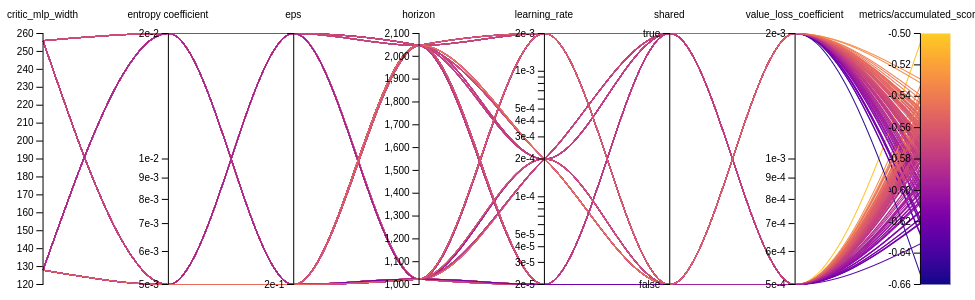
\includegraphics[width=1.0\textwidth]{resources/psppo_sweep.png}
\caption{A graph representing the different combinations and outcomes of the grid search.}
\label{fig:psppo_sweep}
\end{figure}
\newpage
Considering the optimal hyperparameters found with the grid search we carried out a test to compare the performances with and without Rewards Shaping.
We used an environment with malfunctions and different agent speeds, specifically using the following parameters:

\begin{lstlisting}[label={lst:psppo-net-init}]
environment_parameters = {
	"n_agents": 5,
        "x_dim": 16 * 3,
        "y_dim": 9 * 3,
        "n_cities": 5,
        "max_rails_between_cities": 2,
        "max_rails_in_city": 3,
        "seed": seed,
        "observation_tree_depth": 2,
        "observation_radius": 10,
        "observation_max_path_depth": 30,
        "malfunction_parameters": MalfunctionParameters(
            malfunction_rate=0.0075,
            min_duration=15,
            max_duration=50),
        "speed_profiles": {
            1.: 0.25,
            1. / 2.: 0.25,
            1. / 3.: 0.25,
            1. / 4.: 0.25},
}
\end{lstlisting}

Therefore the tests were replicated with seeds: 14, 50, 80, 130, 200 and the final result, for each metric, obtained by making an average.
According to the criteria described in ~\ref{subsec:rewards2} we have chosen the following parameters for testing with Rewards Shaping:

\begin{lstlisting}[label={lst:psppo-net-init}]
environment_parameters = {
        "reward_shaping": True,
        "uniform_reward": True,
        "stop_penalty": -1/n_agents,
        "invalid_action_penalty": -0.0,
        "deadlock_penalty": -n_agents,
        "shortest_path_penalty_coefficient": 1 + 1/n_agents,
        "done_bonus": 1/n_agents,
}
\end{lstlisting}

The basic idea is that deadlocks are more catastrophic, in terms of performances, as the number of agents increases given their irreversible nature.
They not only prevent the agents involved from being unable to move, but also block passages that can be used by other agents to reach the destination.
We have also observed cases where the deadlocks of one part of the agents completely prevented the others from reaching their destination.
So with this parameter configuration for RewardsShaping, we wanted to penalize more deadlocks than  \textbf{$stop\_penalty$}, \textbf{$shortest\_path\_penalty\_coefficient$} and \textbf{$done\_bonus$} which are mainly related to reaching the destination in the least number of steps.
The plots clearly show that RewardsShaping has a positive impact on performance. 
Apparently the only metrics where the no RewardsShaping approach seems to perform better are those concerning deadlocks, however we have noticed that this effect is due to the learning of a polarized policy on the STOP\_MOVING: when an agent is stationary most of the time it is less likely to go into a deadlock and this is also the reason for decreasing trend of the other metrics. \\
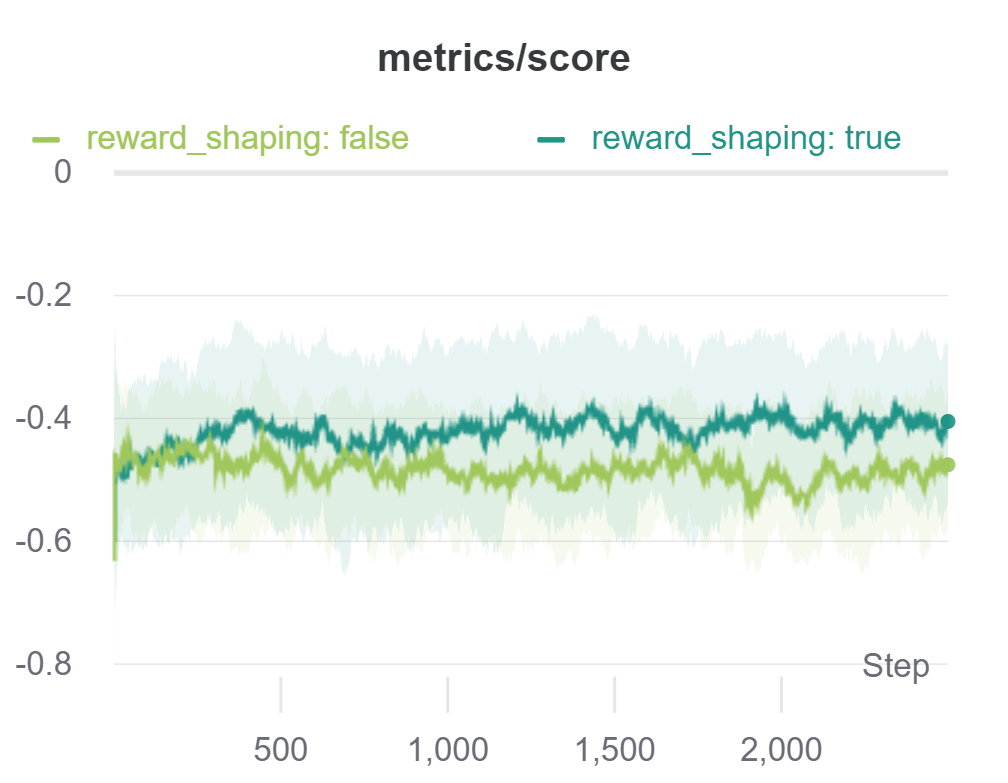
\includegraphics[width=0.33\linewidth]{resources/charts_psppo_1/score}
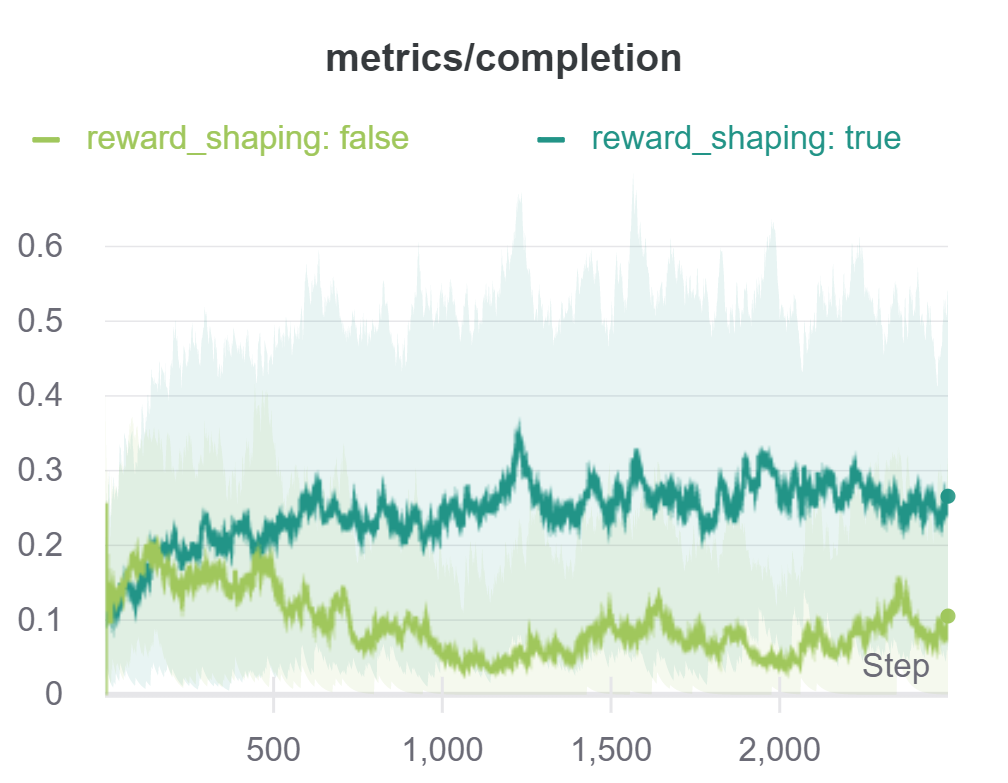
\includegraphics[width=0.33\linewidth]{resources/charts_psppo_1/completion}
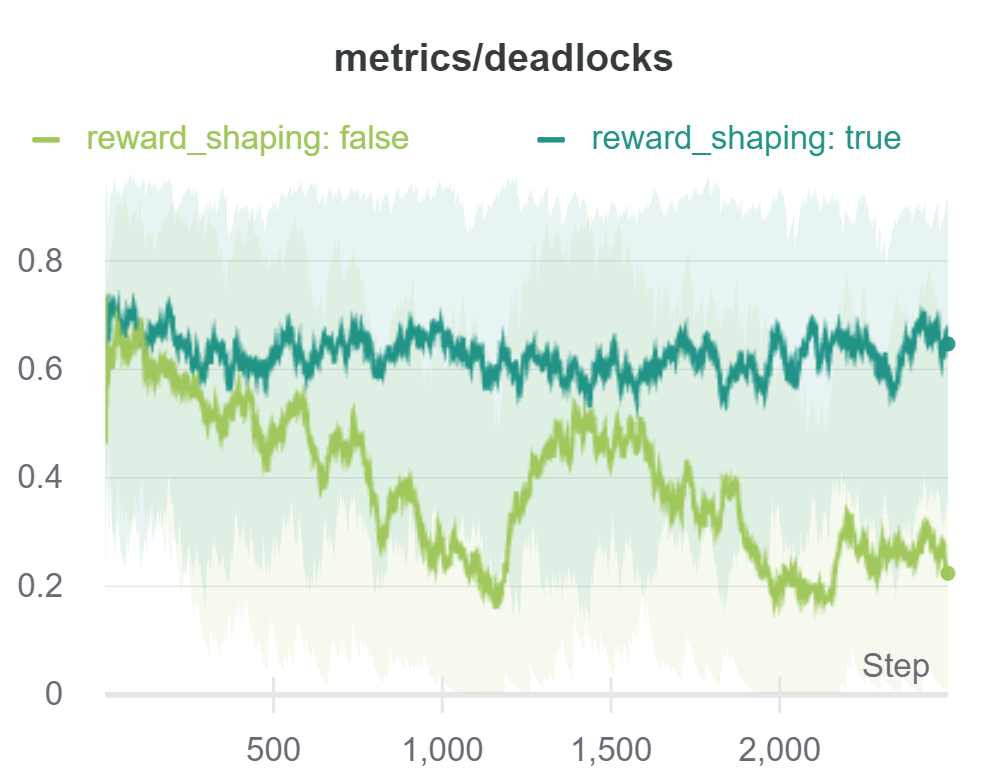
\includegraphics[width=0.33\linewidth]{resources/charts_psppo_1/deadlocks}
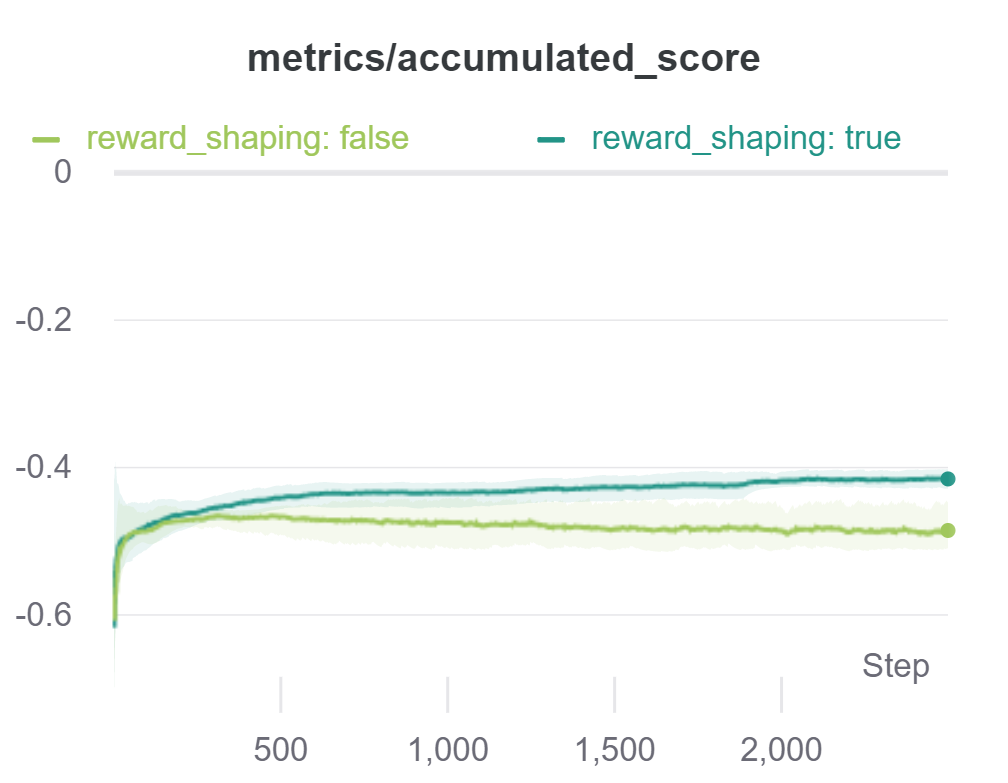
\includegraphics[width=0.33\linewidth]{resources/charts_psppo_1/accumulated_score}
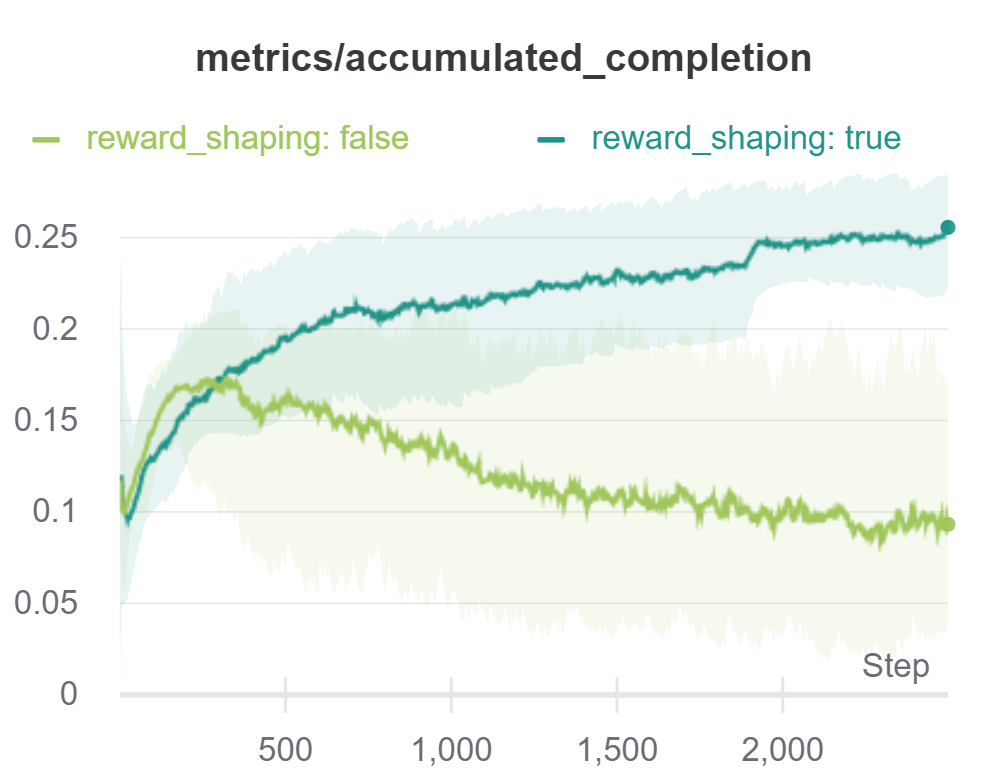
\includegraphics[width=0.33\linewidth]{resources/charts_psppo_1/accumulated_completion}
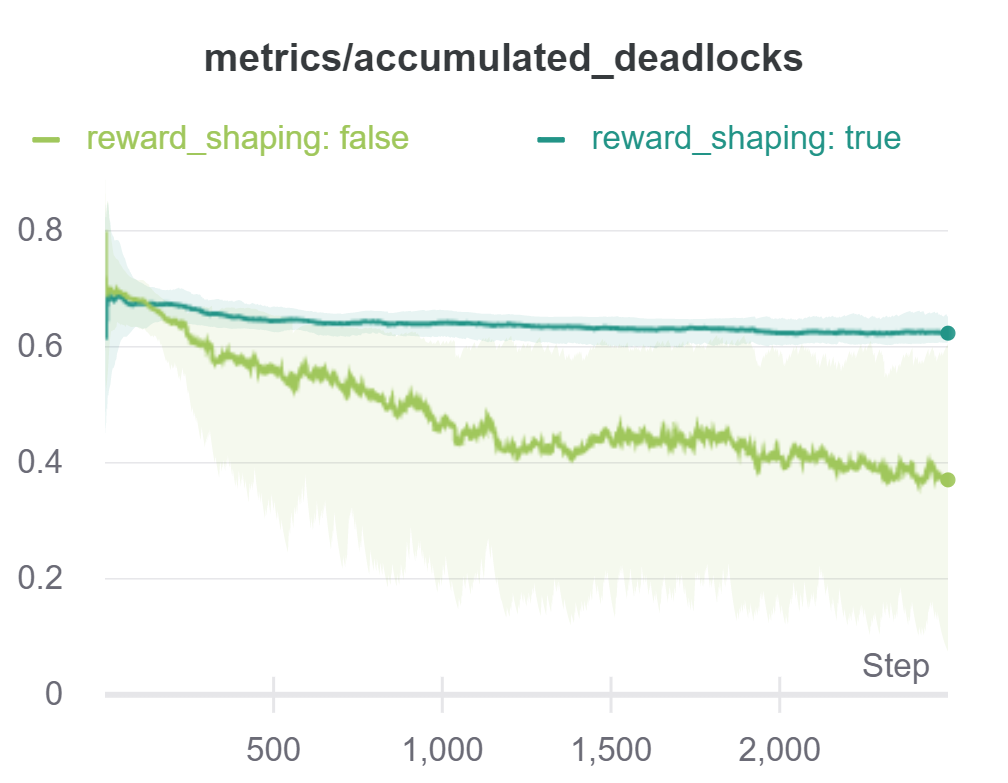
\includegraphics[width=0.33\linewidth]{resources/charts_psppo_1/accumulated_deadlocks}
As it was mentioned in ~\ref{subsubsec:network-architecture} our algorithm provides the possibility to use a Long-Short-Term-Memory (LSTM) module as the shared portion of the network which is well-suited to make predictions based on time series data like the trajectories in a reinforcment-learning problem.
We then repeated the experiment described above by exploiting LSTM, to evaluate its benefits, using the following hyperparameters: 
\begin{lstlisting}[label={lst:psppo-net-init}]
training_parameters = {
        "shared_recurrent": True,
        "linear_size": 128,
        "hidden_size": 64,
}
\end{lstlisting}
Another variant tested arises from a different interpretation of the trajectory of each agent: considering the tuples $(s, a, r, s')$ as belonging to a single episode, if the agent does not reach its destination, in the computation of $GAE$ as it was mentioned in ~\ref{subsubsec:training-setup2}. 
This approach does not seem really correct but brings an improvement in performance as shown in the graphs where:
\begin{itemize}
\item "endtraj-norecurrent" is the best of the test described above.
\item "end-traj-recurrent" is the same test with LSTM.
\item "noendtraj-recurrent" is the test with LSTM with the different interpretation of the trajectory. 
\end{itemize}

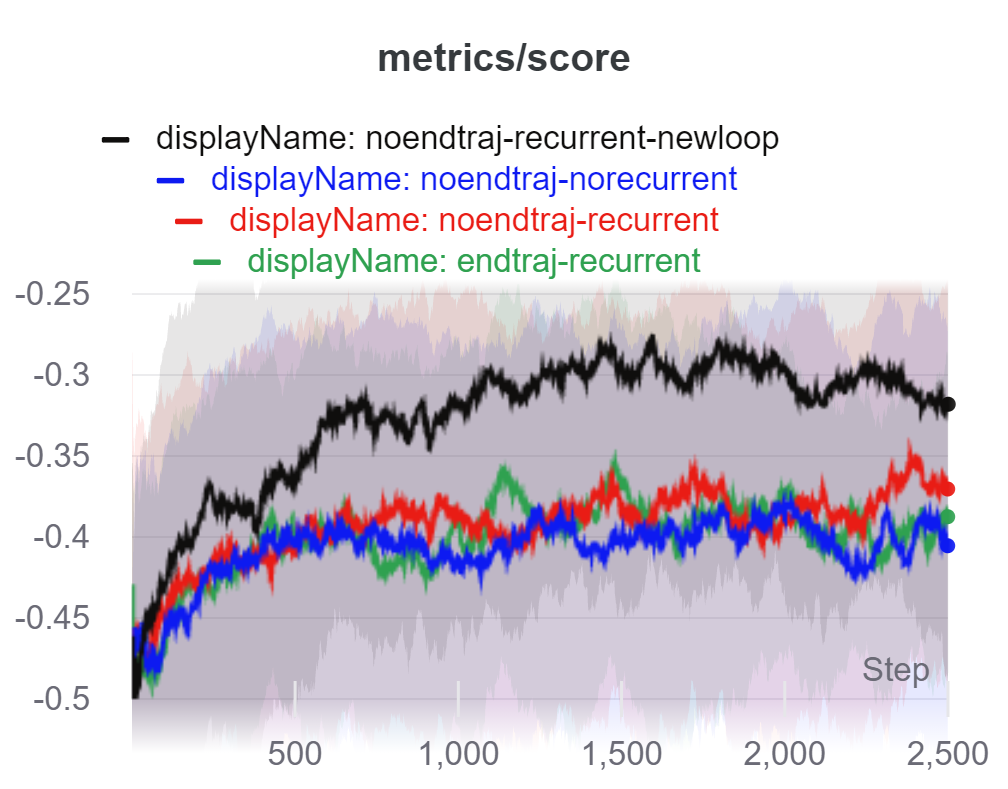
\includegraphics[width=0.33\linewidth]{resources/charts_psppo_2/score}
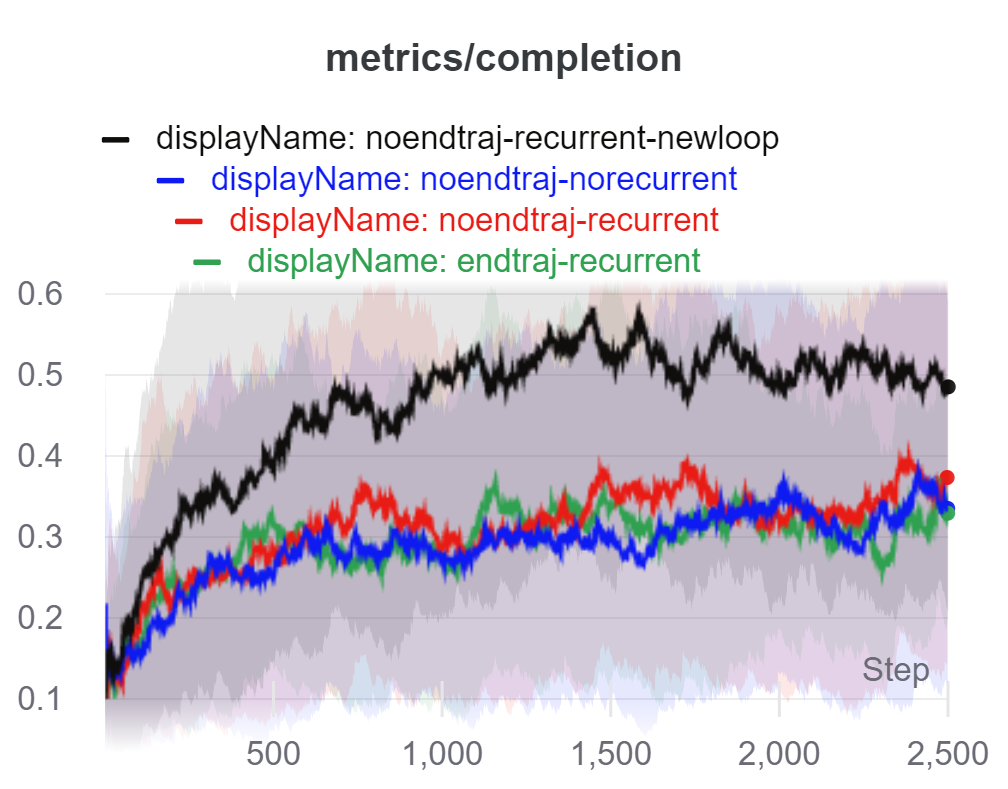
\includegraphics[width=0.33\linewidth]{resources/charts_psppo_2/completion}
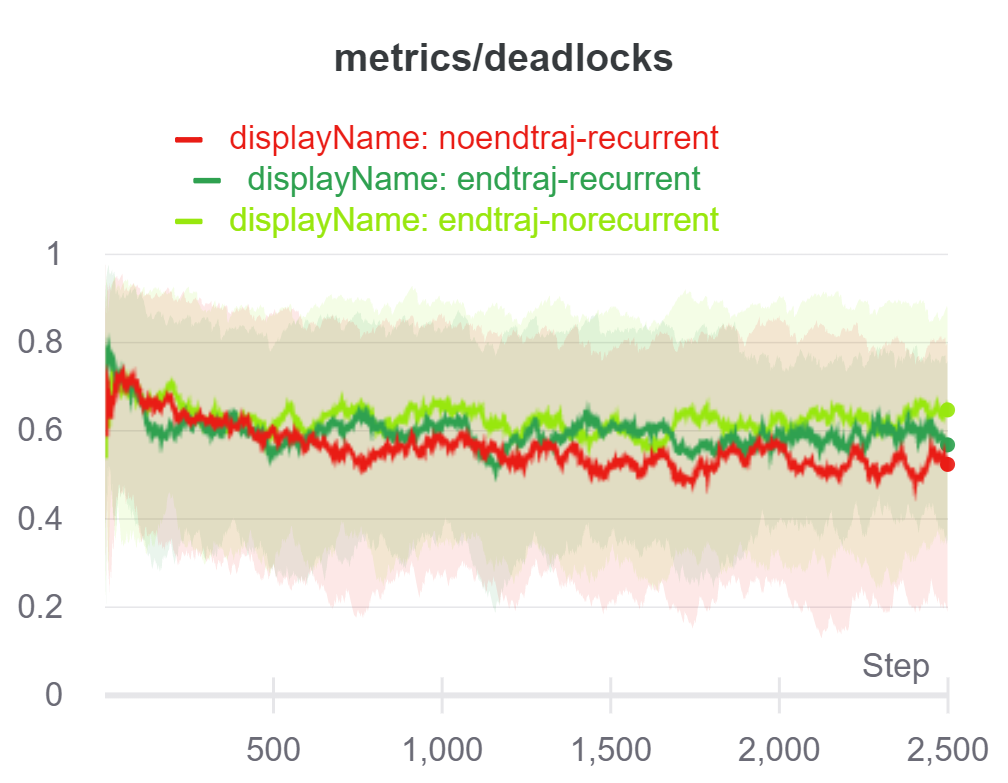
\includegraphics[width=0.33\linewidth]{resources/charts_psppo_2/deadlocks}
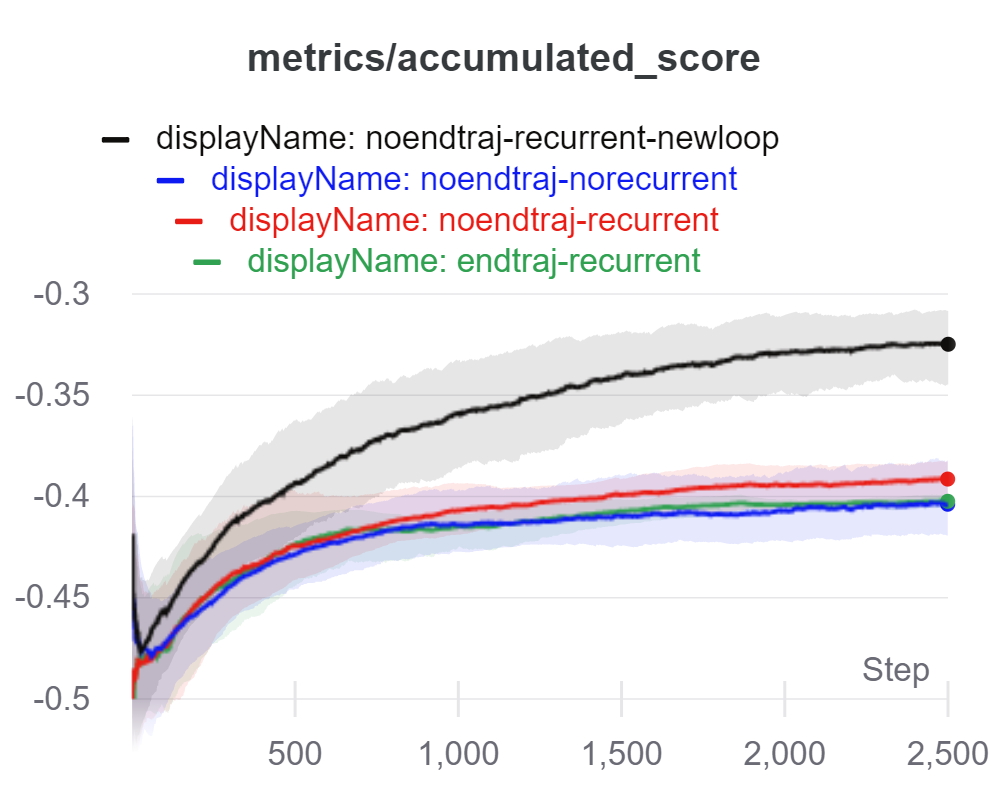
\includegraphics[width=0.33\linewidth]{resources/charts_psppo_2/accumulated_score}
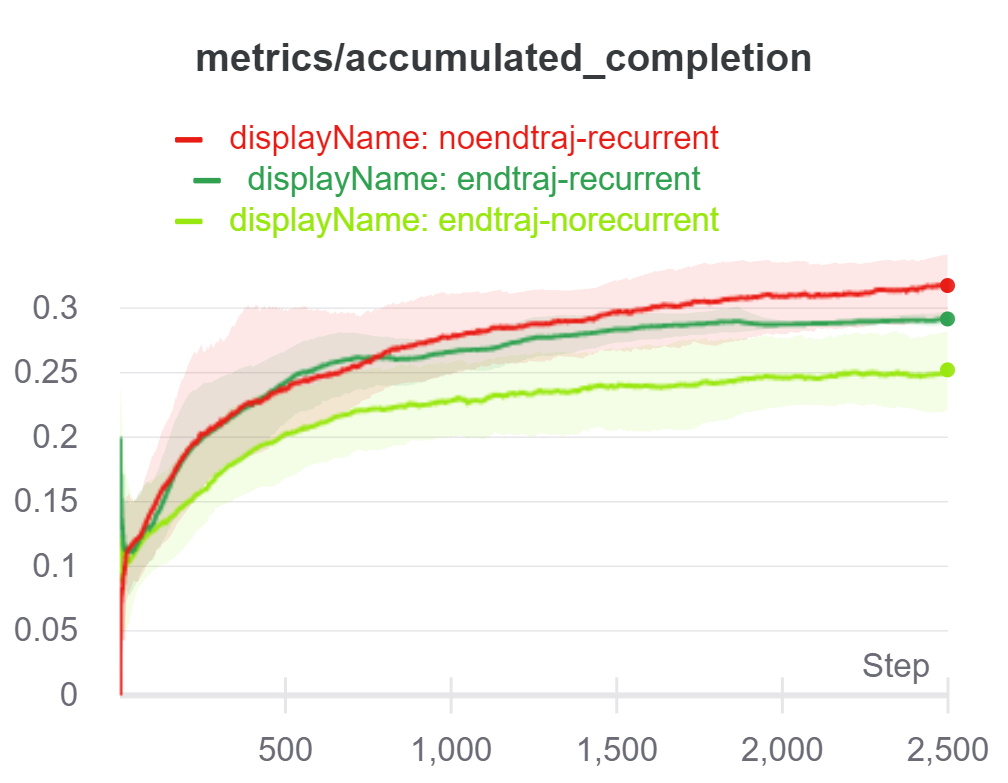
\includegraphics[width=0.33\linewidth]{resources/charts_psppo_2/accumulated_completion}
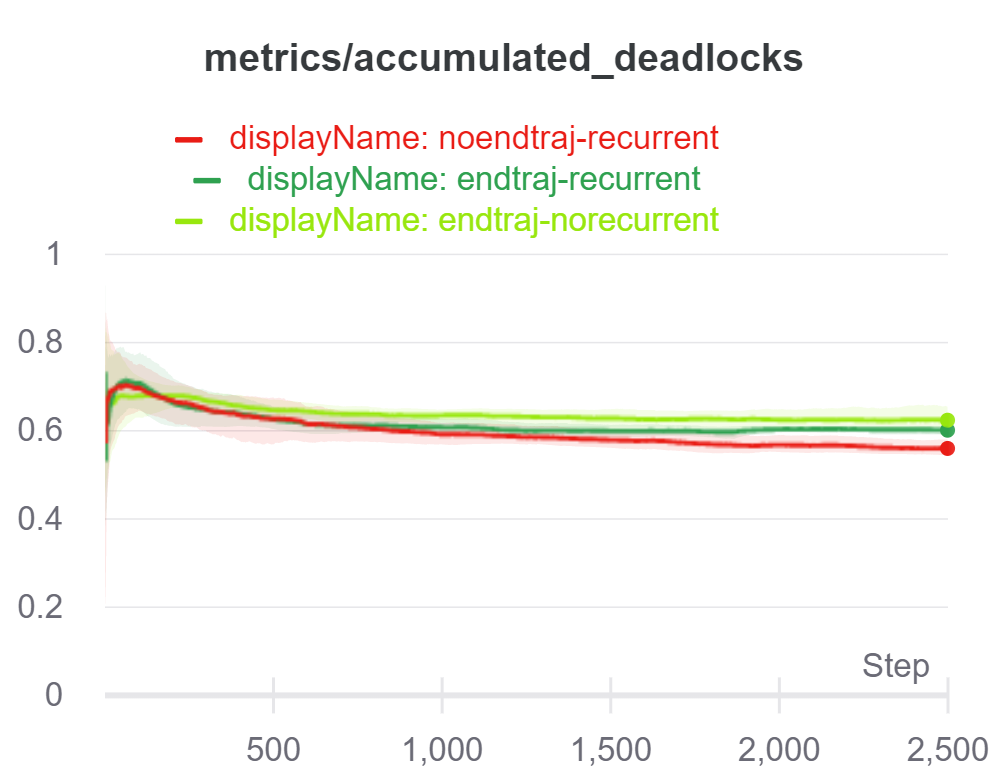
\includegraphics[width=0.33\linewidth]{resources/charts_psppo_2/accumulated_deadlocks}
\section{D3QN}\label{sec:d3qn}

\textbf{Deep Q Networks (DQN)} have been proposed as the union of Deep Learning with Q-Learning to deal with complex and high dimensional environments such as video games and robotics.
In this setting the neural network plays as a predictor from states to Q values, substituting a less scalable table of values.
From the initial work~\citep{dqn} many supplements have been proposed to improve different parts of the original algorithm.
\textbf{Dueling Double Deep Q Networks (D3QN)} represents a combination of many of them.
A very wide overview of the main techniques applied to DQN can be found in~\citep{rainbow}.

\subsection{Algorithm}\label{subsec:algorithm2}

The first D of D3QN stands for Dueling, an idea proposed in~\citep{dueling} which splits the neural network in two parts, one which computes an estimate of the values as usual and another the advantage of each action to understand which states are valuable without exploring the outcomes of each possible action.
For example in the Flatland environment agents does not perform actions which substantially influence the environment, as many of them are moving forward.
In this case, the idea is to increase the training phase and allow the controller to detect and learn how to act in critical positions such as switches.
At the end, advantages and values are combined to obtain Q values.
The second D stands for Double, which refers to the idea of using two separate neural networks during training, one called the primary network, is used to compute Q values used to choose the optimal action, while the other, called the target network, is used to estimate the Q value of the chosen action in the given state.
Double DQN have been recently proposed in multi-agent context in the algorithm \textbf{Weighted Double Deep Q-network (WDDQN)} presented in the work~\citep{weighted-ddqn}.

\begin{figure}
	\begin{gather*}
		\delta = r + \gamma Q\left( s^{'}, argmax_{a^{'}}Q\left( s^{'}, a^{'}; \theta_{k} \right); \theta_{k}^{-} \right) - Q(s, a; \theta_{k})\\\\
	    L(\theta_{k}, \theta_{k}^{-}) = E_{\left(s, a, r, s^{'}\right) \sim D} \left( \delta \right)^{2}\\
	\end{gather*}

	\caption{The objective function of the Double DQN algorithm using a batch of transitions $(s, a, r, s^{'})$ sampled from the experience replay D. $\delta$ is called \textbf{Temporal Difference (TD) Error}, if the state $s$ is terminal $\delta = r$ . $\theta$ represents the parameters of the online network while $\theta^{-}$ the parameters of the target network.}\label{fig:d3qn_objective}
\end{figure}

Our D3QN uses also different experience replay strategies as described in~\ref{subsubsec:experience-replay}.
The mentioned improvements have been proposed in a single-agent scenario, but as already discussed in chapter~\ref{ch:multi-agent-reinforcement-learning} many adaptations to classical RL algorithms have been proposed for multi-agent setting.
The following part will continue describing a soft adaptation to multi-agent scenario inspired by the~\href{https://gitlab.aicrowd.com/flatland/flatland-examples}{Flatland's baselines} which relies mostly on the classical single-agent implementation while~\ref{subsubsec:fingerprints} describes more specific tricks.
We consider the former strategy an "analysis of emergent behaviors" study, as the adaptations to multi-agent setting are minimal and there are low theoretical guarantees even if performances show empirical good results.

\subsection{Implementation}\label{subsec:implementation2}

This section describes the most remarkable details of the algorithm implementation.

\subsubsection{Network architecture}

Similarly to PS-PPO also D3QN allows customization on layers depth and width.
The layers form a fully connected neural network.
As D3QN has a dueling component the network structure is heavily bounded on this choice, after some hidden layers, involved in the encoding of the agent's observation, the network terminates in two branches, one responsible for the computation of action advantages and the other for the state value prediction, the results are aggregated summing the two outcomes and subtracting the mean of the advantage.
Hidden layers weights can be set shared between the two flows or separated.
At the end, two neural networks are declared following the above description.
The two networks work in synergy providing respectively the local and the target of the Double DQN strategy.
The local is updated with gradient descents and used to predict the best action and the Q value of the previous state, while the target receives the best action and computes the Q value of the following state.
The local network is used also to collect trajectories following the the Q values approximations and exploiting the acquired knowledge about the environment, while with a certain probability $\epsilon$ it is forced to choose a random action to affect exploration.
If action masking is active both choices are masked.
This strategy is called \textbf{$\epsilon$-Greedy}, it allows the agents to explore more at the beginning and exploit better after a while, decaying the probability to randomly explore the environment during the training.
The final loss used to optimize the local network is the mean squared error of the discounted Q value of the successive state summed with the reward with the Q value of the current state.
The target network's weights are updated using \textbf{soft updates}, which can be described with the following formula:
\begin{equation}
	\theta^{-} = \theta \tau + \theta^{-}(1 - \tau)\label{eq:soft-update}
\end{equation}
where $\theta^{-}$ are the target's weights, $\theta$ the local network's weights and $\tau$ an hyperparameter usually set to a very small number as this update is performed at each mini-batch gradient descent.
Network graphs can be seen in the figures~\ref{fig:d3qn_uer_graph} and~\ref{fig:d3qn_per_graph}.

\subsubsection{Training setup}\label{subsubsec:training-setup2}

In each episode the agents decide an action whenever they are ready to perform an action, namely they are not already moving from a cell to another, this may also include agents in deadlock which are involuntarily accumulating movements they will never perform, and are not arrived to destination.
Agents that not decide an action perform a DO\_NOTHING action.
Agents which have decided an action save in the experience replay the resulting transitions to form trajectories.
The algorithm here provides a variant (the type 1) to also include transitions of agents arrived at their destination.
When an agent's memory has reached both a minimum fixed size and the batch size, every interval of steps it is filled with a certain amount of transitions it is used to train the agent.
Neural networks are updated with sampled batches of transitions stored in the memory, the different mechanisms of sampling and types of memories are described in~\ref{subsubsec:experience-replay}.
After each episode the exploration rate $\epsilon$ of the $\epsilon$-greedy is decayed with a fixed factor until it reaches a final value set in the hyperparameters.

\subsubsection{Experience Replay}\label{subsubsec:experience-replay}

As mentioned in~\ref{subsubsec:training-setup} one of the most important aspect to consider in a DRL algorithm is the nature of the input given to learn policies or value functions.
Value based methods, such as D3QN, use experience more easily, allowing agents to collect it and reuse it in future learning iterations, this technique is called \textbf{Experience Replay (ER)}.
Samples of batches are drawn from the pool uniformly.
This approach introduce two main benefits: data is reused (sample efficiency) and correlations between randomly sampled steps is lower than using online data.

\begin{quoting}[font=itshape, begintext={"}, endtext={"\citep{human-level}}]
we used a biologically inspired mechanism termed experience replay that randomizes over the data, thereby removing correlations in the observation sequence and smoothing over changes in the data distribution.\\
\[\dots\]\\
In the future, it will be important to explore the potential use of biasing the content of experience replay towards salient events, a phenomenon that characterizes empirically observed hippocampal replay, and relates to the notion of "prioritized sweeping" in reinforcement learning.
\end{quoting}

\textbf{Prioritized Experience Replay (PER)} introduced in~\citep{prioritized}, extends the uniform ER by learning to replay memories where the real reward significantly diverges from the expected reward, letting the agent adjust itself in response to developing incorrect assumptions.
PER implementation can be described in three parts:
\begin{itemize}
	\item The \textbf{SumTree} data structure.
SumTrees are binary trees where each parent node contains the sum of its children.
In this context the tree is used to store data and related priorities inside the leaves while the other nodes are involved in updating more efficiently priorities to speed up samplings and insertions.
	\item The part associated to insertion of new data.
\begin{figure}
	\[ P(i) = \frac{p_{i}^{\alpha}}{\sum_{k}p_{k}^{\alpha}} \]
	\caption{$p_i = |\delta| + \epsilon$ where $\epsilon$ is a small constant ensuring that the sample has a non-zero probability of being drawn. $\alpha$ determines the level of prioritization. If $\alpha$ is near zero, then there is no prioritization, otherwise if $\alpha$ is near 1 sampling data points depends much more on the actual TD errors.}\label{fig:per_priority}
\end{figure}
Before inserting new data, an initial priority must be computed and for each new transition a prediction of the Q value must be computed and compared with the estimation both based on the current value estimator.
A larger difference between the two values, called \textbf{Temporal Difference Error (TD Error)} suggests that more exploration must be done to improve the predictor.
TD Errors and an hyperparameter $\alpha$ are used to compute the probability of each sample.
	\item The part associated to the batch sampling, where \textbf{Importance Sampling Weights} are computed and used to correct the bias introduced by high-priority samples.
\begin{figure}
    \[ w_{i} = \left(\frac{1}{N} \frac{1}{P(i)} \right)^{\beta} \]
	\caption{$N$ is the memory size. The hyperparameter $\beta$ controls how much prioritization is applied. Training is highly unstable at the beginning, and importance sampling corrections matter more near the end of training. Thus, $\beta$ starts small and anneals towards one. Weights are then applied to the TD error $\delta$ in the objective function.}\label{fig:importance_weights}
\end{figure}
\end{itemize}
The consequences on the computational graph of the different methods can be seen in the figures~\ref{fig:d3qn_uer_graph} and~\ref{fig:d3qn_per_graph}.

\subsubsection{Fingerprints}\label{subsubsec:fingerprints}

A condition for ER to be useful is that the environment should not change over time because this makes past experiences irrelevant
or even harmful~\citep{Hernandez-Leal-2019}.
This could be a problem when many agents are concurrently changing and learning in the same environment, due to non-stationarity.
To overcome this problem many methods have been proposed mainly based in associating additional information to the memory's samples to help disambiguation, similarly to what we have done in PS-PPO\@.
Other algorithms that have been already cited, are LDQN, based on leniency of state-action pairs, and WDDQN, which introduces a Lenient Reward Network to approximate lenient rewards.
Other methods rely on expanded experience buffers such as Concurrent Experience Replay Trajectories (CERTS).
A work almost completely focused on dealing with this problem is~\citep{fingerprints}.
In their work Foerster et al.~propose two methods to overcome non-stationarity:
\begin{itemize}
	\item Importance sampling, experience tuples are augmented with the probability of taking the joint action according to the policies at that time.
Sampling of experiences is influenced by the difference between the old and the new environments.
	\item Fingerprints, experience tuples are marked with a temporal countersign, called fingerprint.
This additional information helps agent to better understand in which moment samples have been saved from the environment and understand the policies of the other agents, without sharing them directly, which is much more costly.
An ideal fingerprint is formed by the training step and the $\epsilon$ exploration rate, as it anneals during time.
\end{itemize}

We applied different fingerprints strategies as we noticed that the original "exploration rate and step" was not effective, for example using episodes, alone or combined with $\epsilon$ or all of them.
Results can be found in~\ref{par:d3qn_er_fp_ps}.

\subsection{Testing}\label{subsec:testing2}

D3QN hyperparameters legend:
\begin{itemize}
	\item Network Architecture
	\begin{itemize}
		\item "double\_dqn": if True the neural network estimates the best action with the local network and computes its Q value with the target network, alternatively the target computes directly the Q value and Fixed Q-targets strategy is adopted.
		\item "shared": if True the actor and the critic share the initial and the hidden layers, alternatively they are two separated networks.
		\item "hidden\_size": number of nodes in a hidden layer.
		\item "hidden\_layers": number of hidden layers.
		\item "learning\_rate": called also step size, defines how much the new information updates the old one.
A common value is $0.52e-4$.
		\item "gamma": the discount factor applied to weight the future states, it determines the importance of future rewards.
A common value is $0.99$, $0$ would make the agent "myopic" and $1$ too concerned on long-terms rewards.
		\item "tau": the value responsible for the target network soft-updating.
A common value is $1e-3$
	\end{itemize}
	\item Training setup
	\begin{itemize}
		\item "n\_episodes": number of training episodes.
        \item "eps\_decay": the multiplicative factor used to update the random choice probability of the $\epsilon-greedy$ strategy.
A common value is $0.99$.
        \item "eps\_start": the initial exploration rate $\epsilon$, usually $1.0$
        \item "eps\_end": the final $\epsilon$ value, usually $0.01$
		\item "batch\_size": size of the batch of experiences sampled from the memory.
		\item "buffer\_min\_size": minimum number of samples inside the memory to start learning.
		\item "update\_every": number of fresh samples inserted in the memory to allow the networks learning.
For example assigning $16$ would mean that the 16\textsuperscript{th} new insertion in the memory triggers the network to learn.
	\end{itemize}
	\item Memory
	\begin{itemize}
		\item "buffer\_size": maximum number of samples collectable in the memory.
When overflows occur the oldest data is replaced with the new.
		\item "memory\_type": "per" to choose Prioritized Experience Replay, "uer" to choose Uniform Experience Replay.
	\end{itemize}
	\item Action Masking and allow no-op
	\begin{itemize}
		\item "action\_masking": True to mask invalid actions.
		\item "allow\_no\_op": True to allow the DO\_NOTHING operation.
	\end{itemize}
\end{itemize}

\paragraph{Grid search}\label{par:d3qn_grid_search}
~\newline
\href{https://app.wandb.ai/fiorenzoparascandolo/flatland-challenge-d3qn}{Sweep page}.\\

We performed a grid search to compare different values on random environments to prevent biases induced by seeds.
Obviously the score represents the right parameter to maximize in the search, but we also consider very important the completion as the score is more difficult to interpret.
The search confirmed that double dqn brings better results, and revealed that smaller batch sizes, shorter and shared neural networks, tend to perform better.
Obviously higher learning rates push the model to converge faster, so in these tests we managed to understand better the limits.
The "update\_every" parameter influenced the two metrics differently, high values (32) cause score to increase while low values (16) improved the completion.
The search did not help to choose between larger (256 neurons) or thinner (128 neurons) networks.
The "type 1" variant described in~\ref{subsubsec:training-setup2} definitely performed better, demonstrating that including in memory experience collected from arrived agents is better.

\paragraph{Experience replay, fingerprints and sharing}\label{par:d3qn_er_fp_ps}
~\newline
\href{https://app.wandb.ai/lomb/flatland-challenge-d3qn-er}{Project page}.\\

After a preliminary grid search we performed a series of training tests to evaluate specific implementation details such as the type of experience replay, the usage of fingerprints and sharing networks.
We performed these tests using a set of environments generated with the seeds 14, 50, 80, 130, 200 to obtain a less biased result.
Apparently adding the fingerprints as described in the papers significantly worsen the performances, while using Prioritized Experience Replay slightly improves the run without fingerprints but remarkably improve the metrics of those with fingerprints.
As other fingerprints strategies containing the step continued to perform badly we concluded that feeding a neural network with an input always different as the global timestep, which can be seen as an identifier, can only damage the performance.
On the other hand using values which change slowly as $\epsilon$ and the episode is better.
After some tests we noticed that the "$\epsilon$ and episode" fingerprint performs better than the others.
In particular we can observe different positive trends:
\begin{itemize}
	\item Without fingerprints, the best outcomes are obtained with shared smaller networks (2 $\times$ 128) and batches (32).
In this setting UER slightly overcome PER\@.
Enabling fingerprints with the same configuration maintains a good result, which overcomes the one without fingerprints.
	\item With fingerprints, the best results are obtained with separated bigger networks (3 $\times$ 256) and batches (128).
% TODO: In this setting PER drastically overcome UER\@.
\end{itemize}

\section{Curriculum Learning}\label{sec:curriculum-learning}

\begin{quoting}[font=itshape, begintext={"}, endtext={"\citep{bengio-curiculum}}]
The basic idea is to start small, learn easier aspects of the task or easier subtasks, and then gradually increase the difficulty level.\\
\[\dots\]\\
Deep learning methods attempt to learn feature hierarchies.
Features at higher levels are formed by the composition of lower level features.
Automatically learning multiple levels of abstraction may allow a system to induce complex functions mapping the input to the output directly from data, without depending heavily on human-crafted features.
\end{quoting}

Curriculum learning represents an effective bio-inspired strategy to improve learning.
Training with a curriculum accelerate the speed of convergence and may improve the final model performance.
Designing an efficient and effective curriculum is not always easy, incorrect choices may also affect negatively the algorithm.
To overcome this issue many techniques have been proposed.
Curriculum Learning applied to Reinforcement Learning must consider three different practical aspects: how to generate tasks, how to order tasks based on difficulty and how to perform \textbf{Transfer Learning} from task to task~\citep{narvekar2020curriculum}.
Transfer learning has been studied to speed up the learning by providing some initial knowledge rather than starting from zero, it has been successfully applied on policies, models, value functions and more.
There are multiple paradigms and approaches to implement the aforementioned aspects, for example: tasks can be structured into graphs or sequences, can be automatically or manually generated, can be based on the agent behaviour or not (adaptivity), can be classified in one or more types.

\subsection{Implementation}\label{subsec:implementation3}

Task generation is the problem of producing a set of tasks such that knowledge transfer through them is beneficial.
Most of the methods assume the domain can be parameterized using some kind of representation, where different instantiations of these parameters create different tasks.
For instance the Flatland environment provides many parameters to define the degree of freedom of the domain: the grid size, the number of agents, the rail generation, the scheduling and the malfunction stochasticity.
Following this idea~\citep{object-oriented-mdp} proposed a partially automated task generation procedure based on Object-Oriented MDPs.
Considering the Flatland problem as a single-task problem, we proposed two approaches to generate sequences of intermediate tasks in order of difficulty: a fully manual and a semi-automatic.
Similarly to the configuration proposed by the ML-Agents Unity toolkit (\href{https://blogs.unity3d.com/2017/12/08/introducing-ml-agents-v0-2-curriculum-learning-new-environments-and-more}{Introducing ML-Agents Toolkit v0.2}), in the fully manual curriculum we defined a .yml file specifying the parameters of each level of learning.
The semi-automatic allows the user to specify hyperparameters to influence the environment parameters using linear functions and to program short therm and long therm task repeating to deal with "catastrophic forgetting".
Differently from the manual the semi-automatic is evaluated lazily using Python generators.
An important question when designing a curricula is determining the stopping criteria.
Typically training is stopped when performance on the task or set of samples has converged, but another option is to train on each task for a level number of episodes or epochs.
We decided to measure the completion performance and allow levels to be repeated for a finite number of times unless a certain completion threshold has not overcome.
Defining multiple tasks in Flatland is not easy, we hypothesized tasks such as "reaching the goal", "avoiding deadlocks" and "optimizing the path" which can be respectively measured in therms of percentage of completions, number of deadlocks and normalized score.
The problem of generating environment is not easy too because parameters must be tuned to generate environments with feasible solutions and a coherent generation, as instance the number of agents must be lower than the number of cities or the size of the map can influence the maximum number of cities, rails between and within cities.
One alternative approach is to manually describe ranges of coherent parameter values or levels of difficulty that allows an adaptive and automatic process of task sequencing.

\subsection{Testing}\label{subsec:testing3}
\href{https://app.wandb.ai/lomb/flatland-challenge-ps-ppo-curriculum?workspace=user-lomb}{Project page}.\\

The test was divided in three phases, the first was the application of the semi-automatic curriculum using the five different environments obtained with the seeds 14, 50, 80, 130, 200, the second consisted in training the environments for 3000 episodes and finally the latter evaluating them.

\chapter{Conclusions and future works}\label{ch:conclusions-and-future-works}

Before concluding we propose some interesting efforts and ideas which may be useful for further progress in this work.
\begin{itemize}
	\item \textbf{Meta-Reinforcement Learning (Meta-RL)} applies meta-learning to Reinforcement Learning to enable the rapid training of agents able to generalize never seen problems, making a move towards general AI\@.
Meta-RL is deeply linked with techniques such as curriculum learning, and would be interesting applying it in this scenario.
A well organized introductory overview can be found here~\citep{weng2019metaRL}.
	\item \textbf{Hierarchical Learning} has been proposed to deal with high dimensional action spaces.
Instead of performing a brute force learning as the majority of Reinforcement Learning techniques do this approach groups the low-level actions in high-level actions, such that a task that originally requires thousands of ordered actions to be performed can be described with less, but more general, actions.
We think this idea perfectly suites the Flatland Challenge and its complex environment, as we can notice that learning from scratch induces training the agent with the same low-level actions which do not reflect well how an agent can solve big problems such as collision avoidance and path finding.
More information can be found in this~\href{https://openai.com/blog/learning-a-hierarchy/}{OpenAI blog post}.
	\item Explore other observation methods, in particular \textbf{global graphical observations}, which have been proposed in some works such as~\citep{Stanford2016MULTIAGENTDR}.
	\item \textbf{Action skipping} and \textbf{Agent preempting} to slightly change how the agents interacts with the environment.
Action skipping allows agents to skip deciding actions in cells where there are no choices, for instance long straight rails, consequently rewards must be adjusted.
We noticed that the agents decide always in the same order, this may cause problems as the Flatland internals actually gives more priority to the agents which have decided first, therefore in deadlock avoidance this choice can be crucial.
In the Flatland Baselines can be found also some code related to \textbf{Sparse Rewards} which should be further investigated, maybe introducing \textbf{Curiosity}~\citep{pathakICMl17curiosity}.
\end{itemize}

\newpage

\appendix
\chapter{Appendix}

% Personalize how appendix is numbered
\renewcommand{\thesection}{A.\arabic{section}}

\section{Algorithms}

\begin{algorithm}[H]
	\uIf{agent is in DONE or in DONE\_REMOVED ($1^{\text{th}}$ case)}{
		no reward is computed\\
		\Return{}
	}
	\uIf{agent is in READY\_TO\_DEPART ($2^{\text{th}}$ case)}{
		if the provided action is a MOVE\_* type and the initial cell is free the agent become ACTIVE and is initialized\\
		reward is computed\\
		\Return{}
	}
	\uIf{agent is in malfunction (($3^{\text{th}}$ case))}{
		reward is computed\\
		\Return{}
	}
	\uIf{agent is at the beginning of a cell}{
		update agent.moving considering the observations above depending on the different action types.\\
		\uIf{agent.moving}{
			the wanted action validity is first checked and if it is valid (considering also the possibility to backup from an invalid MOVE\_RIGHT or MOVE\_LEFT to a valid MOVE\_FORWARD) action is stored otherwise agent.moving becomes False and penalties are added, in this process agent.moving and agent.speed\_data['transition\_action\_on\_cellexit'] are updated
		}
	}

	\eIf{agent.moving ($4^{\text{th}}$ case)}{
		Updates the percentage of completion then if it is completely arrived on the next cell, before updating the position, the direction and clears the completion percentage it checks whether the new cell is free. Until the cell remains occupied in the future executions the agent will repeat this process.\\
		reward is computed
	}{
		reward is computed
	}
 	\caption{The \textit{\_step\_agent} algorithm}\label{alg:flatland-agent-loop}
\end{algorithm}
\noindent
\begin{algorithm}[H]
\SetKwFunction{FCheckDeadlocks}{CheckDeadlocks}

\For{$agent$ in range($n\_agents$)}{
	\uIf{agent is ACTIVE and not(deadlocks[agent])}{
		$deadlocks[agent]$ = CheckDeadlocks(agent)
	}
}

\SetKwProg{Fn}{Function}{:}{\KwRet}
\Fn{\FCheckDeadlocks{$agent$}}{
	    $agent\_2 = check\_next\_pos(agent)$ \\
	    if agent is active it is checked whether the cell he will occupy, taking into account his direction, there is another agent. \\
	    If its direction is not valid, i.e. if the cell it is facing is not part of the railway, $check\_next\_pos$ searches in space for possible transitions. \\
            \uIf{$agent\_2$ is $None$}{
 		\KwRet\ False; \\
		if there is no agent in the cell he will take care then $agent$ is not in deadlock.
	    }
	    \uIf{$deadlocks[agent\_2]$}{
		\KwRet\ True; \\
		if agent\_2 was already deadlocked agent is deadlocked too.
	    }
	    \uElse{
		 $deadlocks[agent\_2]$ = CheckDeadlocks(agent\_2) \\
		 If agent\_2 is not deadlocked until the current step, it is checked if it is deadlocked.
	    }
	    \If{$deadlocks[agent\_2]$}{
		\KwRet\ True \\
		if in the current step agent\_2's deadlock is detected then $agent$ is also in deadlock
            }

	    \KwRet\ False
}
\caption{The \textit{deadlocks\_detection} algorithm}\label{alg:deadlocks}
\end{algorithm}

\newpage

\section{PyTorch}\label{sec:pytorch}

This section provides a very briefly overview in FAQ format of PyTorch functionalities and references to more detailed external materials.

\paragraph{What is PyTorch?}\label{par:what-is-pytorch}
PyTorch is an open source machine learning library based on the Torch library.
As deep learning building blocks are tensors similarly PyTorch fundamental class is \textit{torch.Tensor}.
Tensors are data structures that can be placed in a specific device, like a GPU, and can be used to track linear algebra operations whenever the \textit{requires\_grad} property is set to True.
This property is propagated through operations to resulting tensors.
When a tensor is generated from the user, for example the input of a neural network, it does not reference a PyTorch \textit{torch.autograd.Function} responsible for its creation (the \textit{grad\_fn property is set to None}) and is called \textbf{leaf}.

\paragraph{How does differentiation work?}\label{par:what-is-autograd}
Another core component of PyTorch is \textbf{Autograd}, which allows automatic differentiation by recording all the operations performed and replaying them backward to compute the gradients.
Gradients are computed invoking the function \textit{backward()} from a starting point, which must be a scalar value like the mean of the tensor containing the computed batch loss.
Gradients are accumulated, thus before computing new gradients the older are usually zeroed, for example when optimizers are used this is accomplished with the function \textit{zero\_grad()}.
Each time the gradients are computed memory buffers created during the forward step are freed preventing the possibility to repeat other backtracks.
To allow multiple backtracks the option \textit{retain\_graph} must be set True.
It is possible to generate graphical representations of the gradients computations with the function \textit{make\_dot(variable)} of the \href{https://github.com/szagoruyko/pytorchviz}{PyTorchViz} package.
These representations are acyclic graphs that encode a complete history of the computation called \textbf{Computational graphs}, which are procedurally generated in the forward pass, by calling the method \textit{nn.Module.forward()}.
Blue boxes are tensors involved in gradient computation such as neural network's weights, biases and inputs, while gray and green boxes both represent recorded operations in which gradients have been involved, the color green is used to underline the starting point, or root of the tree.
It is possible to prune parts of the computation graph setting Tensor's attribute \textit{requires\_grad} to False, or alternatively in a more temporarily way, enclosing the interested code portions within a \textit{with torch.no\_grad()} block or more permanently detaching tensors from the current graph with the \textit{detach()} method.

\paragraph{What is the difference from PyTorch to TensorFlow/Keras?}\label{par:what-is-the-difference-from-pytorch-to-tensorflow/keras?}
While TensorFlow provides both a low level and high level API, Keras is mainly an high level API and PyTorch a low level one.
PyTorch usually allows much more flexibility but it is also less intuitive and user-friendly than the other libraries.
Probably the most important difference between PyTorch and TensorFlow is the way they define computational graphs.
While Tensorflow creates static graphs, PyTorch deploys \textbf{dynamic graphs}.
Practically this means that in PyTorch it is possible to define/manipulate graphs on the fly rather than following two separate and ordered steps: definition and execution.
Therefore PyTorch neural networks can be easily executed and examined.

\paragraph{How to integrate CUDA?}\label{par:how-to-integrate-cuda?}
To check whether CUDA is available the method \textit{torch.cuda.is\\\_available()} can be called.
To move a Tensor from the CPU to the GPU the method \textit{to(device)} can be used passing as device the text \textit{'cuda:0'}.
It is also possible to assign the device in the definition passing a string to the argument \textit{device}.

\paragraph{How to build a neural network?}\label{par:how-to-build-a-neural-network?}
Neural networks are supported by the package \textit{torch.nn}.
Custom neural networks are built inheriting the PyTorch \textit{nn.Module} class, it is also possible to combine them and call one inside another as a function, for instance the class \textit{nn.Sequential} used in the various Actor-Critic implementations for both parts are declared inside an extension of \textit{nn.Module}.
When a class extends \textit{nn.Module} it should implement the function \textit{forward()} to describe how the different components and layers of the network work together, permitting a lot of flexibility.
\textbf{Parameters} are Tensor subclasses, that are automatically assigned as network parameters (they will appear in \textit{parameters()} iterator) when used with \textit{Module}s.
The package \textit{torch.nn} provides also the implementation of many layers such as Convolutional, Recurrent and Fully Connected.

\paragraph{How to train a neural network?}\label{par:how-to-train-a-neural-network?}
Neural networks can be trained using state of the art optimization algorithms already implemented and available inside the package \textit{torch.optim}, such as RMSProp and Adam.
Optimizers have a common interface and store inside their state to allow a transparent usage.
Usually they are initialized passing the parameters to optimize, such as neural network's weights and biases.
\\
\\
Additional materials, can be found in the \href{https://pytorch.org/resources/}{official site} or in the following blogs and articles \href{https://blog.paperspace.com/pytorch-101-understanding-graphs-and-automatic-differentiation/}{PyTorch 101, Part 1: Understanding Graphs, Automatic Differentiation and Autograd} and \href{https://towardsdatascience.com/understanding-pytorch-with-an-example-a-step-by-step-tutorial-81fc5f8c4e8e}{Understanding PyTorch with an example: a step-by-step tutorial}.

\section{Figures}

\begin{figure}
\centering
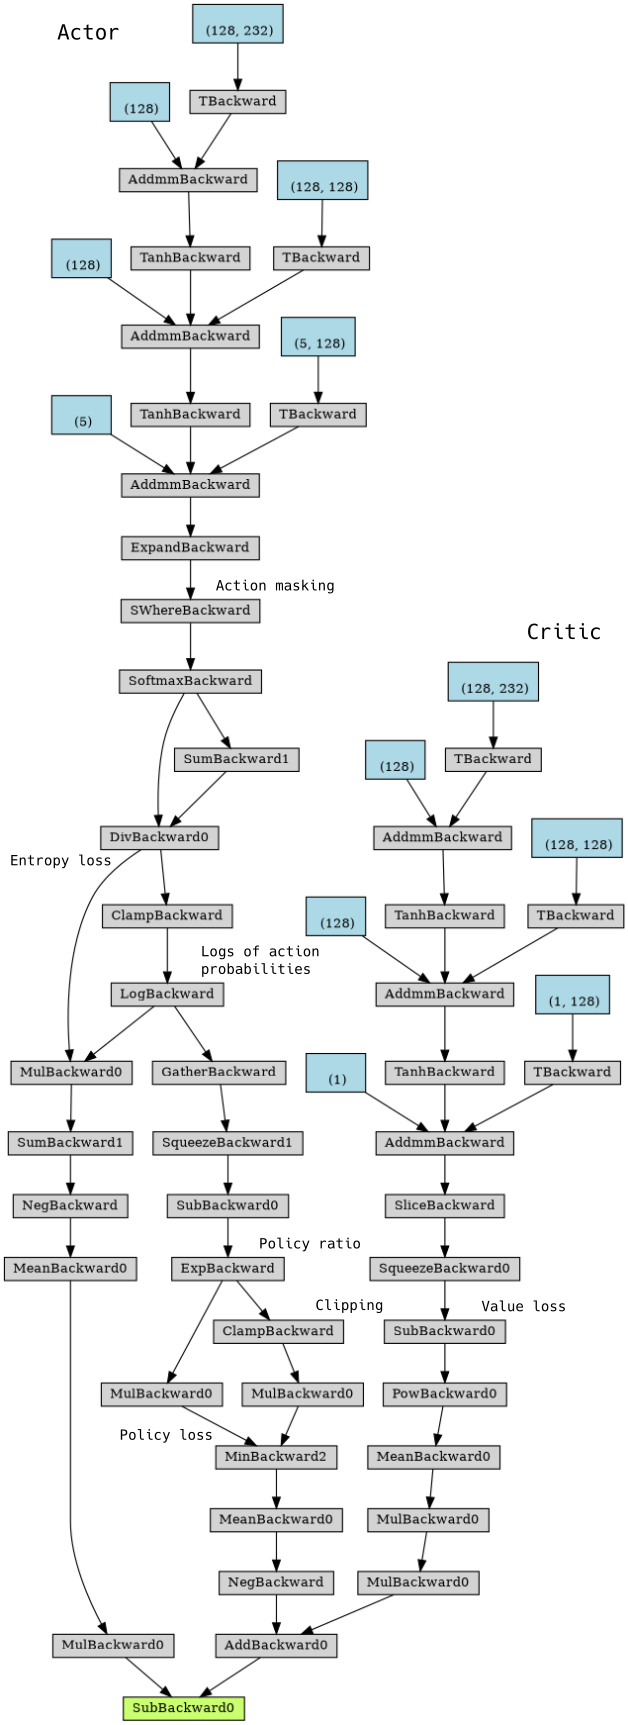
\includegraphics[width=0.46\textwidth]{resources/psppo_separated_graph_commented.png}
\caption{An example of execution graph with actor and critic separated}
\label{fig:psppo_separated_graph_commented}
\end{figure}

\begin{figure}
\centering
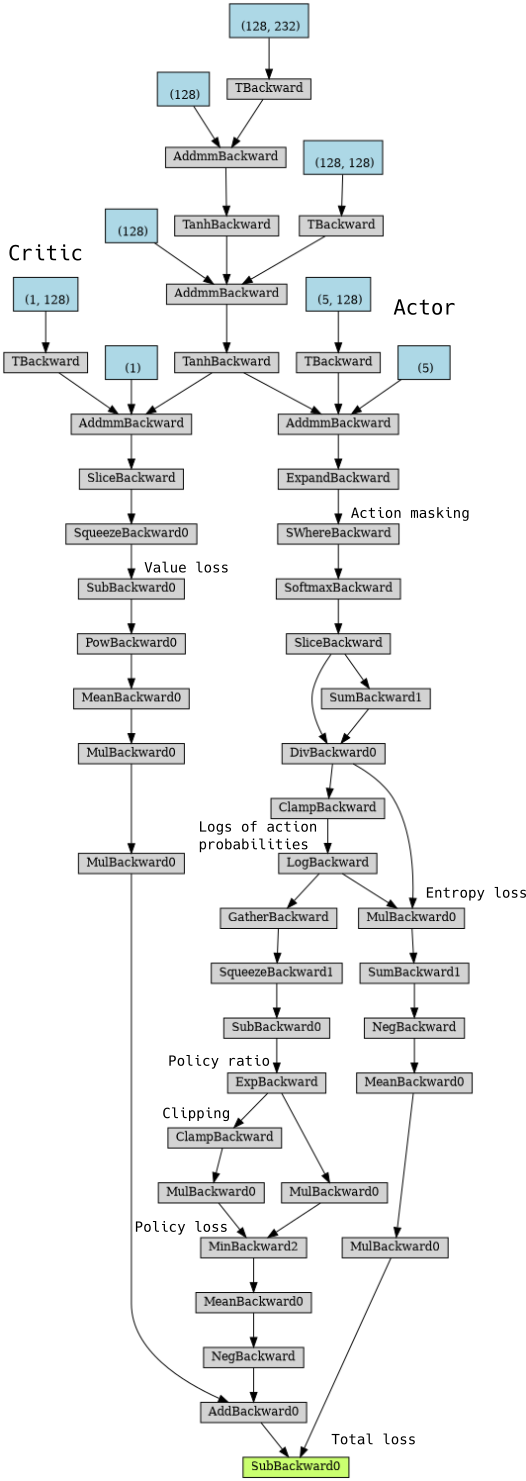
\includegraphics[width=0.45\textwidth]{resources/psppo_shared_graph_commented.png}
\caption{An example of execution graph with actor and critic with shared layers}
\label{fig:psppo_shared_graph_commented}
\end{figure}

\begin{figure}
\centering
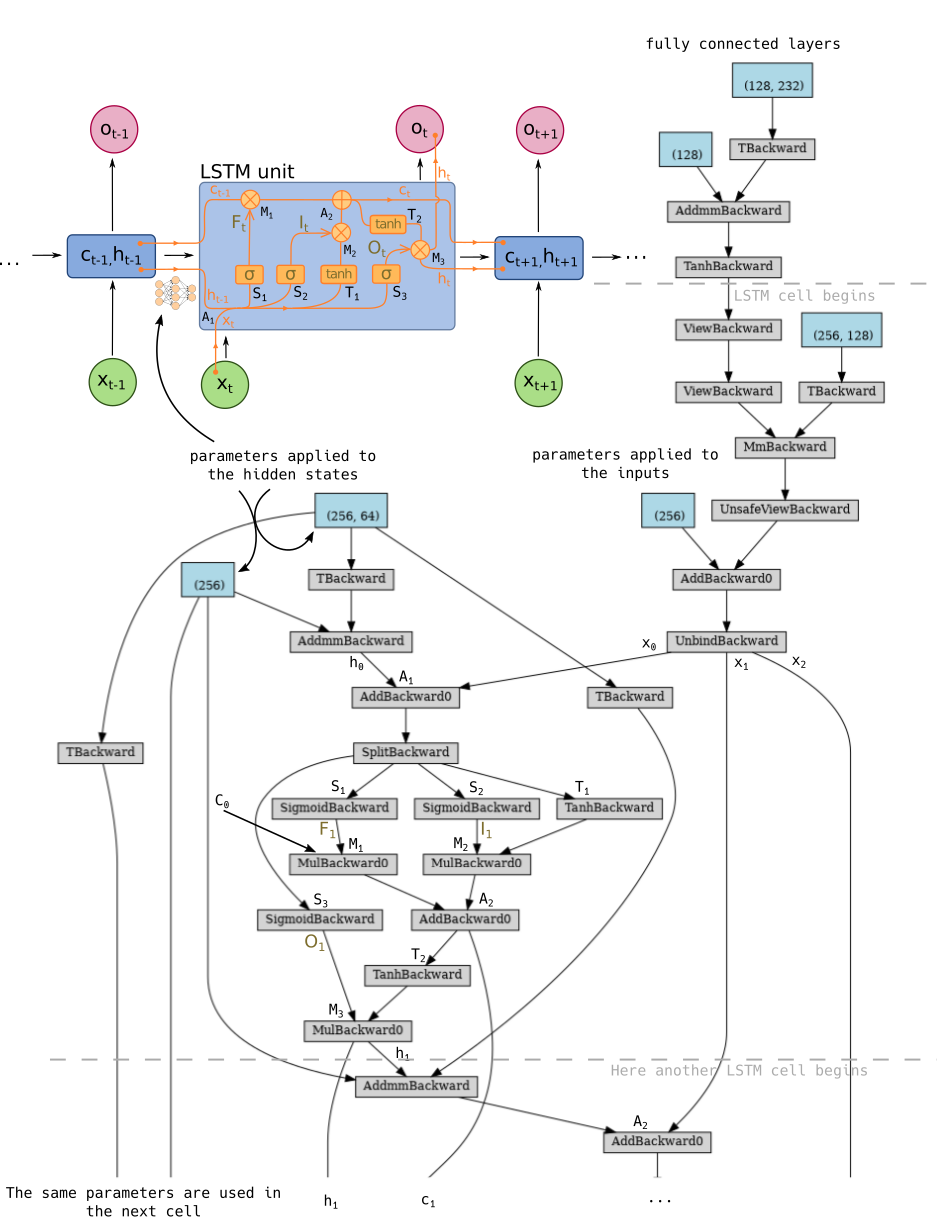
\includegraphics[width=0.925\textwidth]{resources/lstm_pytorch.png}
\caption{A portion of the recurrent PS-PPO computation graph containing a LSTM cell compared with the formal representation.}
\label{fig:psppo_shared_recurrent_graph}
\end{figure}

\begin{figure}
\centering
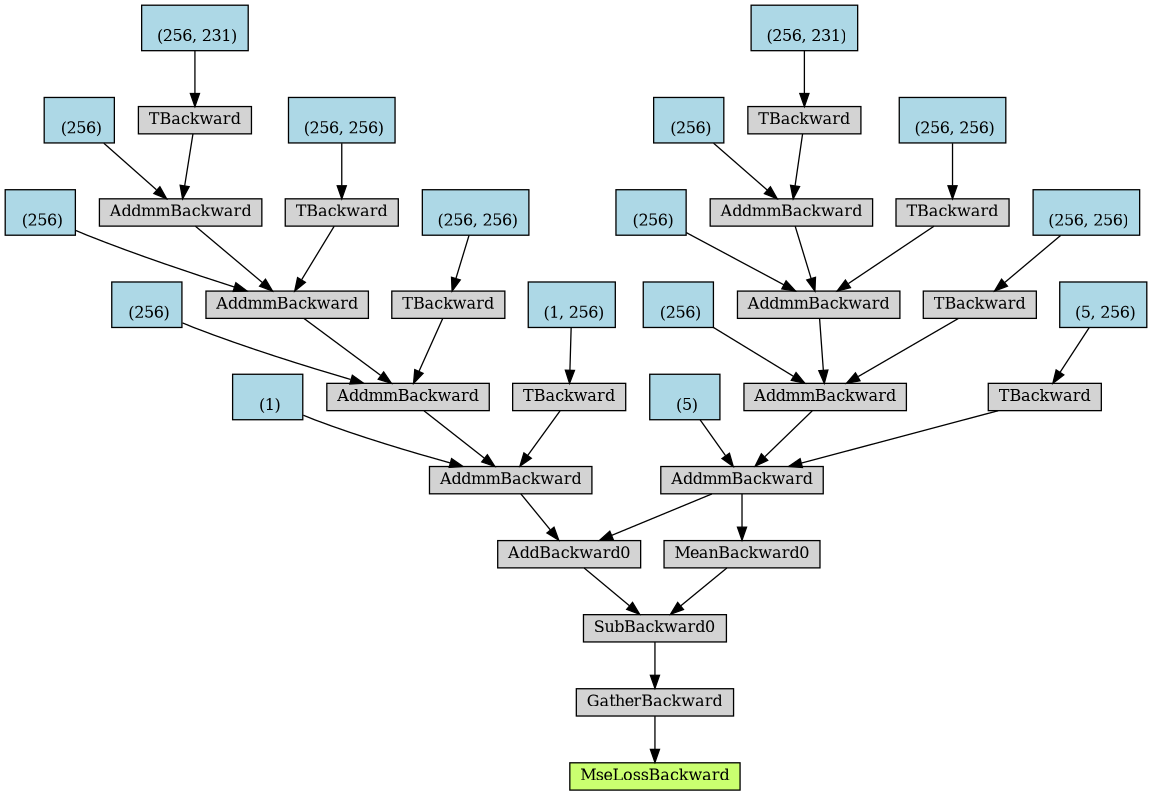
\includegraphics[width=0.74\textwidth]{resources/d3qn_uer_graph.png}
\caption{An example of execution graph with uniform experience replay}
\label{fig:d3qn_uer_graph}
\end{figure}

\begin{figure}
\centering
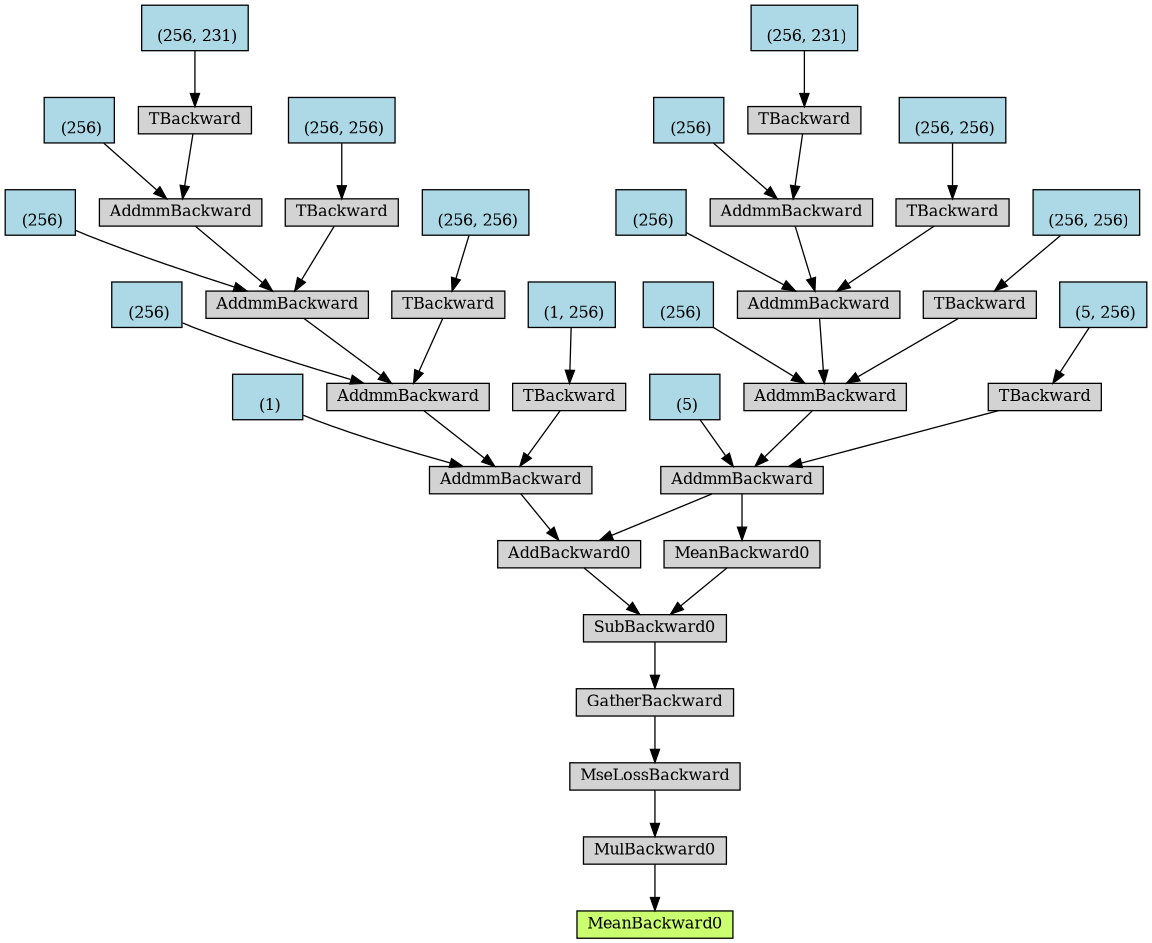
\includegraphics[width=0.74\textwidth]{resources/d3qn_per_graph.png}
\caption{An example of execution graph with prioritized experience replay}
\label{fig:d3qn_per_graph}
\end{figure}

~\nocite{*}
\bibliography{bibliography}


\end{document}
